\documentclass{lkx_thesis}
\usepackage{lkx_thesis}
\usepackage{lkx_diagrams}

\title{Exotic Spheres}
\subtitle{A Geometric Perspective}
\author{Lev Kruglyak}

\department{The Department of Mathematics}
\degree{Bachelor of Arts with Honors}
\subject{Mathematics}

\university{Harvard University}
\location{Cambridge, Massachusetts}
\date{April 2025}

\titlegraphic{graphics/title/e8.jpg}

\advisor{Dr. Stephen McKean}
\advisor{Professor Michael Hopkins}

\begin{document}

\makeatletter
{
	\begin{titlepage}
		\begin{center}
			\hfill
			\vfill
			{\huge\bfseries\scshape\@title}\\[2ex]
			{\Large\@subtitle}\\[1em]

			{
			\scshape
			{by\\[1em]}
			{\bfseries\large\textsl{\@author}}\\[1em]

			{advised by\\[1em]}
			{\bfseries\large\textsl\advisorlist}\\[0.5in]

			\vfill
			\includegraphics[width=3in]{graphics/empty_diagram.png}\\[0.5in]
			\vfill
			{A thesis presented to \\[1em]}
			{\large\textsl{\@university}\\[1em]}
			in partial fulfillment of the\\
			requirements for the degree of\\[1em]

			{
			\large
			{\textsl\@degree}\\
			in the subject of
				{\textsl\@subject}\\[1em]
			}

			{\@location}\\
			{\@date}\\
			}
		\end{center}
	\end{titlepage}
}
\makeatother
\pagebreak


\lkxtoc

% Epigraph
\begin{flushleft}
	\textsl{Existence plays a mischievous game with us,}\\
	\textsl{as though to tease and provoke us. In the }\\
	\textsl{midst of knowledge there yet again arises }\\
	\textsl{the mystery; in the midst of contemplation}\\
	\textsl{the riddle gains new strength.}\\
	\rule[0pt]{19.5em}{0.5pt}\\
	-- \textsc{Rav. Joseph Soloveitchik}\\
	% \phantom{-- }\textsl{``Ish ha'Halakhah''}
	\vspace{2em}
\end{flushleft}

% \begin{flushleft}
% 	\textsl{One might say that, in whatever manner God might have}\\
% 	\textsl{created the world, it would always have been in accordance}\\
% 	\textsl{with a certain general order. But God has chosen the most}\\
% 	\textsl{perfect world, that is, the one which is at the same time}\\
% 	\textsl{the simplest in hypothesis and richest in phenomena.}\\
% 	\rule[0pt]{26em}{0.5pt}\\
% 	-- \textsc{Gottfried Leibniz}\\
% 	% \phantom{-- }\textsl{``Discours de m\'etaphysique''}
% 	\vspace{2em}
% \end{flushleft}

During my last summer before graduating college, some friends and I set out on a mountaineering trip up Banner peak, a picturesque mountain in the eastern Sierra Nevada range of California. Just before the exhaustion of the multiple day trip set in, the conversation turned towards the upcoming year, where I mentioned that I would be writing a senior thesis on exotic spheres.
I struggled to find the words to explain intuitively what these exotic spheres were, much less what made them ``exotic'' in the first place. 
The best I could manage was ``exotic spheres are spaces which are shaped like spheres, but have some twistedness about them which makes them somehow different to spheres''. I mentioned something about how exotic spheres allegedly showed up in some very theoretical physics, so maybe they had applications outside of math?
Compared to the creeping glaciers and massive walls of imposing granite, exotic spheres seemed like a distant and artificial academic oddity. 
While much of my initial hesitation was due to my own lack of understanding of these strange objects at the time, the problem of a simple explanation for an exotic sphere remains. 

One of the reasons for this complexity is that exotic spheres are phenomena which are fundamentally high dimensional in nature. As far as we know, the smallest dimensional exotic sphere is 7-dimensional, far beyond the threshold for a complete visual picture. Another difficulty is that by their very definition, exotic spheres are related to subtle differences in the way we define \emph{space} in mathematics. These subtleties, combined with the high dimensions in which they take place make this a hard subject to visualize. The fact that we are even able to detect and classify exotic spheres at all is a testament to the powerful abstraction achieved by modern mathematics. 

\section*{The Shape of Space}

The simplest, oldest, and arguably most intuitive conceptualization of space is that of Euclidean space -- an infinitely extending flat canvas of points in which parallel lines do not intersect. Most of classical geometry occurred in this context, either in $2$ or $3$ dimensions. 
Less often, mathematicians worked in higher dimensional versions of Euclidean geometry. These were less intuitive and tricker to draw on paper, but the basic geometric rules still applied.
Throughout the 19th century, mathematicians such as Gauss, Riemann, and Lobachevsky began to uncover models of geometry in which many of the assumptions of Euclidean geometry no longer held. 
For instance, using the curved surface of a ball as a canvas for geometry gives fundamentally different results than when using a plane. For starters, parallel ``lines'' on the surface of a ball always intersect (think longitudinal lines on a globe).
More quantitatively, the case of a ball has the sum of angles in a triangle add up to less than $180^\circ$ while in case of a plane the sum of angles in a triangle add up to exactly $180^\circ$. The failure of a triangle's angles to add up to $180^\circ$ or for parallel lines to avoid intersection is an example of \emph{curvature} -- deviation from the flat geometry of Euclidean space.

It's important to note that while geometers had worked with circles, spheres, and other curved surfaces for millenia, they were always embedded in Euclidean space as in the case of a ball in $3$-dimensional space. The novel idea behind non-Euclidean models was that the curved space was \emph{all there was} -- the $2$-dimensional surface of the ball could exist as a geometrical space \emph{independently} of its embedding in $3$-dimensional space. 
The curvature of geometric spaces was not the curving of something \emph{into} an ambient space but rather an intrinsic geometric feature of the sapce itself. After all, measuring angles and drawing lines can be done entirely without leaving the surface of the ball. Even without an understanding of $3$-dimensions, a flat creature living on the ball could conclude that they existed in a curved non-Euclidean space.
By dispensing with the Euclidean axiom of flatness, mathematicians opened up a cornucopia of rich geometry to explore, and these explorations have only grown grander in scope over time.

\begin{figure}[ht]
	\centering
	\todo{draw the figure}
	\medskip
	\caption{Triangles in Euclidean (left) and non-Euclidean geometries.}
\end{figure}

% At the time, many of these new geometries were seen as abstract mathematical departures from the physically motivated notions of Euclidean geometry. Much to everyone's surprise, this all changed with Einstein's theory of general relativity in 1915. Einstein showed that space and time are much better modelled by a non-Euclidean, $4$-dimensional geometry than by a Euclidean geometry, permanently cementing non-Euclidean geometry into the undoubtedly tangible realm of physics.

Near the end of the 19th century, a sparse set of theorems and loose definitions began to consolidate into a field known as topology. Although there weren't many clear definitions in the early days of the field, the central idea was simple. Rather than just removing the axiom of flatness like in the case of non-Euclidean geometries, topology removes most of the axioms, leaving only the \emph{shape} of space, detached from any quantitative information. Unlike a geometric space, a topological space does not come with any notions of distance, angle, perpendicularity, area or volume -- all that is left is a notion of continuity. 
In the geometry that most people are familiar with, two shapes are said to be congruent, or geometrically equivalent, if we can transform between them in a way that does not alter distances,angles, and consequently areas. 
The only requirement for a topological equivalence is that it is continuous, that is, close together points in the first shape should be close together after the transformation. More informally, ripping the shape is not allowed, but any squishy deformation is totally fine. Such a transformation is known as a \emph{homeomorphism} -- coming from Greek roots for ``similar shape''.
\begin{figure}[ht]
	\centering
	\import{graphics/temp-diagrams/}{congruence-vs-homeomorphism.pdf_tex}
	\caption{Geometric equivalence (congruence) vs topological equivalence (homeomorphism)}
\end{figure}

In many areas of topology, we require our spaces to be \emph{manifolds}.
A space is said to be a manifold if it can be built out of patches of coordinate space. For instance, our intuitive model of the surface of the earth is flat, specified by the perpendicular directions -- north/south and east/west. On human scales, this coordinate system is indistinguishable from a flat plane. However, if we keep going north we'd end up at the north pole, at which point the notion of ``further north'' no longer makes sense. At the north pole, we'd have to come up with a different coordinate system but that's fine -- as long as a space has a local coordinate system at each point, the space is a manifold. The number of coordinates needed to describe a manifold is known as its \emph{dimension}. The surface of the earth for example can be represented by a two-dimensional manifold, this is a two-dimensional sphere. Similarly, a circle can be thought of as a one-dimensional manifold since locally it looks like a line, a circle can be thought of as a one-dimensional sphere.
A three-dimensional sphere is a bit harder to visualize, but is still within the realm of human imagination. Remember, the surface of the Earth is a two-dimensional sphere which is embedded in three-dimensional space. My favorite way to visualize a three-dimensional sphere is by a sort of ``dumpling'' construction. blah blah \todo{not sure if this is needed}
\begin{figure}[ht]
	\centering
	\todo{building spheres by pinching}
	\medskip
	\caption{A ``dumpling'' construction.}
\end{figure}

\todo{I have a written section on Riemann surfaces and Poincar\'e's simplicial complexes but it might be too much of a detour}

While the study of manifolds is a deep and fascinating discipline in itself, many manifolds have some extra geometric structure which makes them more interesting to work with. Many of these structures were originally inspired by physics.
% In the very early days of topology for instance, 
% Poincar\'e worked largely with manifolds built up of small triangles, tetrahedra, and their higher dimensional analogues. 
% By counting the number and intersections of these small pieces, Poincar\'e was able to develop a theory of ``combinatorial topology''. \todo{talk about Euler number}
\todo{talk about symplectic manifold -> classical mechanics?, Riemannian geometry for Einstein}
The common feature behind all of these geometric structures was that they required a notion of ``calculus'' on manifolds, i.e. infinitesimals, derivatives, and the like. Mathematicians did what they do best -- remove unnecessary axioms and work primarily in this most general context. For calculus on manifolds, the most general definition was that of a \emph{smooth structure}, the word smooth here meaning ``infinitely differentiable''. In the spirit of topology, while a smooth structure might not allow you to get precise numerical solutions to differential equations, it does allow you to explore the dimensionality of the solutions -- how many \emph{types} of solutions are there rather than what exactly they are. Instead of only requiring two equivalent manifolds to just have the same shape, we now also require equivalences between them to be infinitely differentiable -- so no infinitely sharp kinks or bends. These smooth equivalences are called \emph{diffeomorphisms}.

With just topology, the dressing room of a manifold is dizzyingly vast.
A circle could be represented by homeomorphism with a square, a squiggly blob, a spiky star, a horrifically jagged fractal snowflake, or literally any other closed loop drawn without lifting your pencil. Any of these outfits ``fit'' the abstract topological circle.
Adding a smooth structure onto a manifold downsizes its walk-in closet of possible representations to a tiny travel suitcase, eliminating any outfits which are not ``smooth''. 

\section*{So what is an Exotic Sphere?}

As with any construction in mathematics, we can ask if (a) a smooth structure always exists on a manifold, and (b) if a smooth structure is unique (at least up to diffeomorphism). The reasonable guess would be yes to both of these questions. After all, how topologically twisted can a manifold get for it not to have a smooth structure at all? Remember, ordinary manifolds still locally look like ordinary Euclidean space. Surely any jaggedness can be smoothed out? If you're drawing a closed loop on a sheet of paper and it comes out jagged, you can always redraw it and hold your pen tighter, the resulting shape would still be the same. Similarly, if you're building a clay model and the surface is rough, you can always gently brush over it with water to get a nice smooth surface. You certainly wouldn't expect smoothing it one way to result in a fundamentally different smooth structure than if you smoothed it a different way. Remember, we're not changing the shape here, the underlying manifold is still the same!

Our intuition is correct in these low-dimensional cases -- in fact every one, two, and three-dimensional manifold admits a unique smooth structure. However, much to our surprise this completely breaks down in dimension four. There, it's possible to construct a manifold which \emph{admits no smooth structure at all}. Even more surprising things happen when we restrict to the case of spheres. Spheres of any dimension have at least one smooth structure -- we can always draw a sphere in Euclidean space and do calculus there. However, this smooth structure is not unique! 
Any time we find a smooth structure on a sphere which is not diffeomorphic to the ordinary one, we call such a sphere \emph{exotic}.
On the seven-dimensional sphere for instance, there are exactly \emph{twenty-eight} distinct smooth structures, no more no less.
One of these corresponds to the ordinary smooth structure, but the rest are all exotic spheres.\footnote{\todo{orientation double counting}}
Next up in dimension, an eight-dimensional has only two smooth structures, while a nine-dimensional sphere has eight smooth structures. In fact, the only dimensions in which a unique smooth structure is know to exist are $1,2,3,5,6,12,56,$ and $61$. This seems oddly specific.
At first glance, the number of smooth structures on the sphere does not appear to follow an obvious pattern.
\begin{figure}[ht]
	\renewcommand{\arraystretch}{1.2}
	\centering
	\begin{tabular}{r|c|c|c|c|c|c|c|c|c|c|c|c|c|c|c}
		\textrm{dimension:} & 1 & 2 & 3 & 4 & 5 & 6 & 7 & 8 & 9 & 10 & 11 & 12 & 13 & 14 & 15\\
		\hline
		\textrm{\# of smooth structures:} & 1 & 1 & 1 & ? & 1 & 1 & 28 & 2 & 8 & 6 & 992 & 1 & 3 & 2 & 16526\\
	\end{tabular}
	\medskip
	\caption{The number of smooth structures on the spheres.}
\end{figure}

When I first heard about exotic spheres in an introductory class on differential topology, I wondered if these were ``real'' mathematical objects or simply quirky artifacts of our definitions. There is of course, no objective answer to this question, and any answer reflects a level of mathematical bias.
As the Prussian mathematician Leopold Kronecker once remarked ``God created the integers, all else is the work of man''. My own philosophy didn't go quite as far as Kronecker's.
I was fairly convinced that non-Euclidean geometries were real -- or at the very least, were more than just a mathematical curiosity.
After all, Einstein's theory of general relativity showed that the space and time of our universe is far better modelled by a curved, $4$-dimensional, non-Euclidean geometry than by a Euclidean geometry. 
The predictive success of Einstein's theory cemented non-Euclidean geometry into the undoubtedly tangible realm of physics. 
Compared to the rigid structures of geometry, the sea of all possible topological spaces is chaotic and vast. Somehow, restricting space to be spherical \todo{something something}


\section*{Ramifications of Exoticity}

\todo{mention how exotic spheres can be thought of as knots, talk about torsion phenomena}


%
% \begin{figure}[ht]
% 	\centering
% 	\todo{cube, icosahedron, vs donut}
% 	\medskip
% 	\caption{The Euler number of polyhedra.}
% \end{figure}
%
% Riemann on the other hand, was interested in functions of a complex variable -- think $f(z)=\sqrt{z}$ where $z$ is allowed to be any complex number. Riemann noticed that some functions such as the square root were ``multivalued''. After all, when $z^2=4$, $z$ could be either equal to $+2$ or $-2$. It would be nice if function had a well-defined value, but a problem arises when you try to choose a ``branch'' of the function -- in this case either positive or negative. As you go around the complex plane, no matter which convention you choose, at some point you will have to switch branches and this causes a discontinuity. Riemann discovered that functions such as the square root are more naturally interpreted as a function on a surface (a two-dimensional manifold) rather than on a flat plane.
% \begin{figure}[ht]
% 	\centering
% 	\todo{riemann surface}
% 	\medskip
% 	\caption{The Riemann surface for $f(z)=\sqrt{z}$.}
% \end{figure}
% This led to his theory of Riemann surfaces, and to later generalizations of the notion of a \emph{complex structure} on a manifold -- i.e. some extra data which allows one to work with complex variables and functions.

% \medskip


% rigor of angels
%
% shape of space
%

% Before talking about exotic spheres, I want to talk about symmetry.

% Projective plane analogy with torsion (Z/2 vs Z/28)

% Humanity has been fascinated by questions of physical space for thousands of years. As with many areas of math, this burning curiosity first arose in antiquity out of practical concerns: measuring the volume of a cylindrical grain silo, computing the circumference of the earth, predicting the motion of celestial bodies, etc. In order to make these questions precise in the idealized world of mathematical forms, we must first make our intuitive notions of space precise. 
% Euclidean geometry, for instance, takes place on an infinite continuum of points, and comes with a way to measure distances and angles. It also contains a strong notion of parallelism -- starting at a point and choosing a direction gives a straight line which extends indefinitely. If we pick any other point not this line, travelling in that same direction gives us a parallel, non-overlapping line.
%
% To us, physical space at the scales which we inhabit is so intuitively Euclidean, and so baked into the very structures of our mind that it's difficult to imagine where our assumptions might be biased. We tend to think of space as infinite and flat, just as Euclid's axioms describe. At the scale of daily life this is an accurate model, but at the scale of the Earth it completely falls apart. The Earth is neither infinite nor flat, and \emph{any} straight line path will eventually bring you back to your starting point. 
% And that's only the two-dimensional surface of the spherical Earth. What if the universe itself was finite, curving in on itself rather than extending indefinitely? You might imagine zooming into the depths of the cosmos with a super-powered telescope only to see familiar galaxies, and eventually Earth itself peering back at you.
% Even worse, what if space was non-orientable? Not only could flying in a straight path bring you right back to where you started, but you would find that upon your arrival the very notions of right and left seem to have swapped places -- as though you've entered a mirror world. All languages become illegible to you since they are now backwards from your perspective, a birthmark which used to be on the left side of your face appears to everyone else to be on your right. Only another trip along the same course you originally took is able to flip everything back.


\chapter{Introduction}\label{chap:introduction}
\begin{flushleft}
	\textsl{There is geometry in the humming of the strings,}\\
	\textsl{and there is music in the spacing of the spheres.}\\
	\rule[0pt]{21em}{0.5pt}\\
	-- \textsc{Pythagoras}\\
	\vspace{2em}
\end{flushleft}

The basic objects of study in differential topology are smooth manifolds. Loosely speaking, smooth manifolds are spaces which locally look like Euclidean space of a given dimension and contain additional ``smooth structure'' which makes it possible to do calculus on them.

\begin{definition}
\end{definition}

\todo{physics and math}

% A smooth structure gives rise to tangent spaces -- at each point of the manifold there is a notion of infinitesimal direction, and the set of all such infinitesimal directions forms a vector space of tangent vectors. \todo{physics}

While the class of smooth manifolds offers a tempting pasture for the exploration of the shape of space, it is far from the only type of manifold one can define. Another equally valid category in which to study topology of manifolds is $\PL$, or the piecewise linear category. A $\PL$ structure on a manifold consists of 

\section{The Generalized Poincar\'e Conjecture}

\begin{conjecture}[Poincar\'e Conjecture]
 Every closed topological $3$-manifold which is simply connected is homeomorphic to the $3$-sphere $S^3$.
\end{conjecture}

\begin{conjecture}[Generalized Poincar\'e Conjecture]
  Letting $\mathscr{C}$ be either $\Top$, $\PL$, or $\Diff$, any $\mathscr{C}$-manifold which is homotopy equivalent to the $n$-sphere $S^n$ is also $\mathscr{C}$-isomorphic to $S^n$.
\end{conjecture}

\subsection{Smooth Tricks of the Trade}

\begin{theorem}[$h$-cobordism]\label{thm:h-cobordism}
  Let $n\geq 5$ and $\mathscr{C}$ be either $\Top$, $\PL$, or $\Diff$. If $M$ and $N$ are $\mathscr{C}$-manifolds and $W : M \hbord N$ is an $h$-cobordism between them, then $W$ is $\mathscr{C}$-isomorphic to the cylinder $M\times [0,1]$.
\end{theorem}

\todo{Reeb theorem, morse theory, conclude with looking for homotopy spheres.}

% \todo{define PL, Diff, Top etc, show differences for instance cone construction}
%
%
%
%
%
% \begin{definition}
%   A closed oriented (smooth) $n$-manifold $M$ is called a \defn{homotopy sphere} if it has the homotopy type of the $n$-sphere $S^n$. An \defn{exotic sphere} is a homotopy $n$-sphere which is not diffeomorphic to the standard $n$-sphere $S^n$.
% \end{definition}
%
% \subsection*{Why is this complicated?}
%
% Any homotopy sphere is \defn{stably parallelizable} -- meaning the stable isomorphism class of its tangent bundle is trivial.
%
% \begin{theorem}
%   If $\Sigma$ is a homotopy $n$-sphere, then $\T \Sigma \oplus \underline{\R}$ is trivial. 
% \end{theorem}
% \begin{proof}
% \end{proof}
%
% In fact, a much stronger result holds true.
% \begin{theorem}
%   If $\Sigma$ is a homotopy $n$-sphere with $f : S^n \to \Sigma$ the homotopy equivalence, then there is a bundle isomorphism $f^*\T\Sigma \approx \T S^n$.
% \end{theorem}
% \begin{proof}
% \end{proof}
%
% \subsection*{Groups of Homotopy Spheres}
%
% See \cite{milnor1963groups} and \cite{levine1985lectures}
%
% \begin{definition}
%   Let $\Theta_n$ denote the group of diffeomorphism classes homotopy $n$-spheres under the operation of connected sum.
% \end{definition}
%
% \begin{definition}
% \end{definition}
%
% \begin{definition}
%   Let $\bP_{n+1}$ denote the subgroup of $\Theta_n$ of (classes of) homotopy $n$-spheres which bound parallelizable manifolds.
% \end{definition}
%
% \begin{theorem}[Kervaire-Milnor]
%   The group of homotopy $(4k-1)$-spheres bounding parallelizable manifolds is a cyclic group of order:
%   \[
%     |\bP^{4k}| = 2^{2k-2}(2^{2k-1}-1)\varepsilon_k\cdot \mathrm{num}(B_{2k}/4k) 
%   \]
% \end{theorem}
%
% \subsection*{The Kirby-Siebenmann Class}
%
% \begin{theorem}
%   For $n\geq 5$, there is an isomorphism $\pi_n(\pl/\diff)\approx \Theta_n$.
% \end{theorem}
%
% \subsection*{Global Gravitational Anomalies}
%
% See \cite{witten1985global}.


\chapter{Detecting Exotic Spheres}\label{chap:detection}
\begin{flushleft}
	\textsl{A mathematician is a blind man in }\\
	\textsl{a dark room looking for a black cat}\\
	\textsl{which isn’t there.}\\
	\rule[0pt]{15em}{0.5pt}\\
	\textsl{-- Unknown}
	\vspace{2em}
\end{flushleft}

In \cref{chap:construction}, the plumbing theorem gave us a surjective map
\[
		b_k : \Z \lkxsurj \bP^{4k}
\]
which constructs a homotopy sphere bounding a parallelizable manifold of signature $8t$ for any $t\in \Z$. By the first isomorphism theorem, it follows that $\bP^{4k}\cong \Z/t_k$ for some $t_k\in \Z$. In this chapter, we'll determine this number $t_k$ and hence derive a formula for the number of exotic $(4k-1)$-spheres bounding parallelizable manifolds. 

There are two avenues of exploration here. The first approach is to use theorems from index theory to construct invariants on $\bP^{4k}$ which can distinguish two homotopy spheres by their signatures. While this approach is beautiful and can detect many exotic spheres, it only gives lower bounds on $t_k$ and is unable to achieve a full classification. A better, although harder approach is to directly compute the kernel $\ker b_k$. We'll see how to do this in \cref{sec:milnor-kervaire-theorem}. As there are many insights gleamed in the first approach, let's begin here.

\section{Characteristic Classes}
\todo{should this be here or in appendix?}

\subsection{Stiefel-Whitney Classes}
\subsection{Chern Classes}
\subsection{Pontryagin Classes}

\begin{proposition}\label{prop:pontryagin-class-of-complex-projective-space}
	The total Pontryagin class of complex projective space is given by
	\[
		p(\CP^n) = (1+\alpha^2)^{n+1}\mod \alpha^{n+1},
	\]
	where $\alpha$ is the degree $2$ generator of the cohomology ring $\H^\bullet(\CP^n)\cong \R[\alpha]/(\alpha^{n+1})$.
\end{proposition}

\subsection{Chern-Weil Theory}

\section{The Hirzebruch Signature Theorem}

Let's understand the signature of a manifold on a deeper level, since it is of such fundamental importance to the structure of $\bP^{4k}$. \todo{historical note} It turns out that the signature of a manifold can be completely expressed in terms of the Pontryagin numbers of the manifold, and the subtleties of this connection leads to many non-trivial results about the integrality of rational expressions involving Pontryagin numbers. The first observation about signature which we could make is:

\begin{proposition}
	If $X$ is the boundary of a manifold $W$, then $\sigma(W)=0$.
\end{proposition}
\begin{proof}
\end{proof}

This has an immediate consequence. If $X$ is a disjoint union $X_1\sqcup (-X_2)$ which bounds a manifold $W$, then it follows that $\sigma(X_1\sqcup (-X_2))=\sigma(X_1)-\sigma(X_2)=0$ so that $\sigma(X_1)=\sigma(X_2)$ (It should be fairly clear that the intersection form of a disjoint union splits as a direct sum so the signature is additive). 
This is exactly the notion of oriented cobordism!

\begin{proposition}
	$\sigma(X_1\times X_2) = \sigma(X_1)\times \sigma(X_2)$.
\end{proposition}

\begin{corollary}
	The signature of a manifold is thus a ring homomorphism
	\[
		\lkxfunc{\sigma}{\Omega^\SO_{\bullet}}{\Z.}
	\]
\end{corollary}

Furthermore, this ring homomorphism factors through the rational cobordism ring as a map \[\Omega_\bullet^\SO\otimes \Q \lkxto \Z\] since torsion elements of $\Omega_\bullet^\SO$ must be mapped to $0\in \Z$. Fortunately for us, we already know the structure of $\Omega_\bullet^\SO\otimes \Q$ -- it is a polynomial ring in $\Q$ generated by the cobordism classes of $\CP^{2k}$. Since the signature of $\CP^{2k}$ is $1$ we can, at least in principle, compute the signature of any closed oriented manifold. Given a closed oriented manifold $M$ and a cobordism decomposition of it as a sum of a torsion component $T$ and products of complex projective planes, the signature of $M$ will count the number of homogeneous monomials in this decomposition.
\[
	M\sobord T\sqcup \bigsqcup_{i\in I} \CP^{2k_{i,1}}\times\cdots \times\CP^{2k_{i,\ell_i}}
	\quad\implies\quad
	\sigma(M) = |I|.
\]
The signature isn't the only integer-valued cobordism invariant out there. The Pontryagin numbers of an closed oriented manifold also depend solely on the cobordism type of the underlying manifold. For the complex projective spaces,

\subsection{Multiplicative Sequences and Genera}

\todo{write about the structure of $\Omega_\bullet^\SO$, Thom-Pontryagin construction, multiplicative sequences, genera, etc}

\begin{definition}
	The \defn{$\bm{L}$-genus} $\{L_k\}$ is the multiplicative sequence of polynomials corresponding to the series $Q(z) = \sqrt{z}/\tanh\sqrt{z}$.
\end{definition}

\begin{theorem}[Hirzebruch]\label{thm:hirzebruch-signature-theorem}
	Let $X$ be a closed $4k$-manifold. Then we have
	\[
		\sigma(X) = \int_X L_k(p_1, \cdots, p_k)(X),
	\]
	where $L_k$ is the $L$-genus.
\end{theorem}
\begin{proof}
	It suffices to check this identity for the generators $\CP^{2k}$. The total Pontryagin class of $\CP^{2k}$ is $p(\CP^{2k})=(1+\alpha^2)^{2k+1}$. Using multiplicativity of $L$ and $L(1+z)=\sqrt{z}/\tanh\sqrt{z}$, we have
	\[
		\begin{aligned}
			L(p)(\CP^{2k})
			= L\left((1+\alpha^2)^{2k+1}\right)
			= L(1+\alpha^2)^{2k+1}
			= \left(\alpha/\tanh \alpha\right)^{2k+1}
			\quad\in\H^\bullet(\CP^{2k}).
		\end{aligned}
	\]
	Here, we consider $\alpha/\tanh \alpha$ as a formal power series in $\alpha$ truncated by the relation $\alpha^{2k+1}=0$ in the cohomology ring $\H^\bullet(\CP^{2k})$. The characteristic number $L_k(p_1,\ldots,p_k)[\CP^{2k}]$ is then the coefficient of $\alpha^{2k}$ in the expansion of $(\alpha/\tanh \alpha)^{2k+1}$.
	By elementary complex analysis, this coefficient can be extracted by taking a contour integral around a small $\varepsilon$-circle about the origin in $\C$:
	\[
		\begin{aligned}
			L_k(p_1,\cdots, p_k)[\CP^{2k}]
			 & = \frac{1}{2\pi i}\oint_{S^1_\varepsilon} \frac{dz}{z^{2k+1}} \left(\frac{z}{\tanh z}\right)^{2k+1}
			 &                                                                                                       \\[0.5em]
			 & = \frac{1}{2\pi i}\oint_{S^1_\varepsilon} \frac{dz}{\tanh^{2k+1} z}\quad
			 & u  =\tanh(z),\quad
			du =(1-u^2)dz
			\\[0.5em]
			 & = \frac{1}{2\pi i}\oint_{S^1_\varepsilon} \frac{1}{u^{2k+1}}\cdot\frac{du}{1-u^2}
			 &                                                                                                       \\[0.5em]
			 & = \frac{1}{2\pi i}\oint_{S^1_\varepsilon} \frac{1+u^2+u^4+\cdots}{u^{2k+1}}\,du                       \\[0.5em]
			 & =1.                                                                                                 &
		\end{aligned}
	\]
	Since $\sigma(\CP^{2k})=1$, this completes the proof.
\end{proof}

The Hirzebruch signature theorem is a shining example of a truly remarkable theorem in mathematics -- it gives us easy computational means to uncover highly non-trivial relationships between complicated objects. For us, the most useful consequence of the Hirzebruch signature theorem is that it gives us subtle integrability and divisibility theorems. For instance, with relatively little effort we can calculate a few $L$-genus polynomials to get:
\begin{equation}\label{eq:L-genus}
	\begin{aligned}
		 & L_1 = \frac{p_1}{3},\quad
		 & L_2 = \frac{7p_2 - p_1^2}{45},\quad
		 & L_3 = \frac{62p_3 - 13p_1p_2 + 2p_1^3}{945},\quad\cdots
	\end{aligned}
\end{equation}
Having done this, the expression for the leading coefficient of $L_3$ in \cref{eq:L-genus} immediately implies:
\begin{corollary}
	If $X$ is a closed $12$-manifold with trivial $\H^4(X)$, then $\sigma(X)$ is divisible by $62$.
\end{corollary}
The observation that for such manifolds $X$, the quantity $\sigma(X)/62$ is an integer, let alone equal to $945p_3[X]$, is far from obvious, and yet it pops out immediately from the signature theorem. These subtle relationships are immensely useful in defining invariants capable of detecting exotic spheres as we will see in the following \cref{sec:constructing-exotic-sphere-invariants}.

While we're on the topic of the $L$-genus, let's compute its leading coefficient. Often times, the manifolds which we'll apply the signature theorem to will be connected enough that the lower order Pontryagin classes vanish -- leaving just the leading term.
Luckily for us, the coefficient of this leading term admits a simple description in terms of the \defn{Bernoulli numbers} $B_{2k}$, a sequence of rational numbers which appear ubiquitously throughout topology, homotopy theory, number theory, and many other disciplines. There are many conventions in the literature, but for our purposes we can define them as the terms appearing in the series expansion of $\tanh z$:
\begin{equation}\label{eq:tanh_series}
	\tanh z = z - \frac{z^3}{3} + \frac{2z^5}{15} - \frac{17z^7}{315}+\cdots = \sum_{k\geq 1} (-1)^k\frac{2^{2k}(2^{2k}-1)B_{2k}}{(2k)!}\, z^{2k-1}.
\end{equation}
With this definition, the first few Bernoulli numbers are given:
\begin{equation}\label{eq:bernoulli_numbers}
	B_0 = 1,\quad B_2 = \frac{1}{6},\quad B_4 = \frac{1}{30},\quad B_6=\frac{1}{42},\quad B_{8}=\frac{1}{30},\quad B_{10} = \frac{5}{66},\quad\cdots
\end{equation}

\todo{complexity of the sequence indicates how complicated the geometry can get}

\begin{proposition}\label{prop:leading_coefficient_L_genus}
	The leading coefficient of the $L$-genus is $s_k=2^{2k}(2^{2k-1}-1)B_{2k}/(2k)!$
\end{proposition}
\begin{proof}
	\todo{this proof}
\end{proof}

\section{Constructing Exotic Sphere Invariants}\label{sec:constructing-exotic-sphere-invariants}

Armed with the power of the Hirzebruch signature theorem, let's now try to build some invariants for the homotopy spheres in $\bP^{4k}$.
Many of the invariants discussed thus far in this thesis have been defined entirely out of the intrinsic geometric and topological data of a manifold. 
Due to the topological simplicity of homotopy spheres, it's difficult to imagine how we could construct such an invariant which can distinguish smooth structure. One of the great ideas of 20th century topology is to pass to a coboundary in situations like this. Namely, if the usual invariants vanish on a manifold $X$, find a manifold $W$ a dimension higher which has $X$ as a boundary (this isn't always possible!). In this case, $W$ is referred to as a \defn{coboundary} of $X$. If we are careful, we can use the topology and geometry of $W$ to construct an invariant which does not depend on the choice of $W$. This is exactly what we will do for exotic spheres in this section. We are in a particularly good position to try this idea since every homotopy sphere in $\bP^{4k}$ necessarily has a coboundary along with a parallelism of the coboundary.

\begin{remark}
	This idea of passing to a coboundary is an example of constructing a \defn{secondary invariant}. When primary invariants, in this case characteristic forms, turn out to be zero, we lift to a case where they are not zero, and use the descent data to measure ``how'' the original invariants vanished. This is a central idea of Chern-Simons theory \cite{chernsimons1974geometricinvariants}, a topic which has found widespread application in constructing quantum field theories. \todo{(?) write more about this?}
\end{remark}

\subsection{Smooth Invariants of Manifolds with Boundary}\label{sec:smooth-invariants-of-manifolds-with-boundary}

Before we can define secondary invariants, we need a good generalization of characteristic numbers to the case of manifolds with boundary. Recall that we need 

\todo{discussion about why topological invariance fails with boundary absent additional restrictions.}

This requires understanding smooth invariants of manifolds with boundary, and this will be the focus of the section.
Throughout let's assume $X$ is a closed $n$-manifold with oriented coboundary $B$.
First of all, we'll note that many \emph{topologically} defined invariants generalize naturally to the case of manifolds with boundary. For instance, the Euler characteristic can be defined as a topological invariant at least for any finite CW complex.
Generalizing the intersection form and correspondingly the signature requires a slight generalization of the Poincar\'e duality theorem:

% \begin{theorem}[Poincar\'e-Lefschetz Duality]
% 	Suppose $X$ is an $n$-dimensional manifold with boundary $\partial X$. Given a fundamental class $[X, \partial X]\in \H^{n}(X, \partial X)$, there is a duality isomorphism
% 	\[
% 		\lkxfunc{}{\H^k(X, \partial X)}{\H_{n-k}(X)}{\omega}{\omega\frown [X,\partial X]}
% 	\]
% 	given by cap product with the fundamental class.
% \end{theorem}
% \begin{proof}
% 	See Theorem~18.6.1 in \cite{dieck2008algebraic}.
% \end{proof}
% As in the case of ordinary Poincar\'e duality, the isomorphism $\H_0(X)\approx \R$ allows us to interpret the cap product as integration when $\omega$ is top dimensional -- there is an isomorphism $\H^m(X)\to \R$ which sends $\omega$ to $\int_X \omega$.
%
% This allows us to define the signature and intersection form of a $4k$-dimensional manifold with boundary.
%
% \begin{definition}
% 	If $X$ is an $4k$-manifold with boundary $\partial X$, the (relative) \defn{intersection form} is the symmetric bilinear form given by
% 	\[
% 		\lkxfunc{I_{X}}{\H^{2k}(X, \partial X)\otimes \H^{2k}(X, \partial X)}
% 		{\R}{\alpha\otimes \beta}{\int_X \alpha\smile \beta.}
% 	\]
% 	The (relative) \defn{signature} $\sigma(X, \partial X)$ of $X$ is the signature of this bilinear form.
% \end{definition}

\begin{convention*}
	Most of the literature simply uses the notation $\sigma(X)$ even when $X$ has a non-empty boundary, and we will adopt this convention outside of this chapter. However, in this chapter, we would like to keep the distinction meaningful for better clarity.
\end{convention*}

While there are no topological constraints on a manifold in order to generalize the signature or Euler characteristic, constraints do appear when generalizing characteristic forms to the relative setting.
Characteristic forms are not a priori relative cohomology classes, so pulling them back to obtain \emph{relative} characteristic forms in order to integrate requires additional assumptions about the topology of the boundary $X$.
For any integer $\ell$, the pair $(B, \partial B) = (B, X)$ gives us a long exact sequence of cohomology groups
\begin{equation}\label{eq:relative_characteristic_classes_exact_sequence}
	\H^{\ell-1}(X) \lkxto \H^{\ell}(B, X) \lkxto[j] \H^{\ell}(B) \lkxto \H^{\ell}(X)
\end{equation}
where $j : \H^{\ell}(B, X) \to \H^{\ell}(B)$ is the induced map of the inclusion $(B,\emptyset) \to (B, X)$. This is an isomorphism if the groups on either side of \cref{eq:relative_characteristic_classes_exact_sequence} are trivial. In this case, we can pullback:

\begin{definition}\label{defn:relative_characteristic_form}
	Suppose that $\H^{\ell}(X)$ and $\H^{\ell-1}(X)$ are trivial. For a characteristic form $c_\ell(B) \in \H^{\ell}(B)$, the \defn{relative characteristic form} is the pullback
	\[
		c_\ell(B, X) = j^{-1} c_\ell(B) \quad\in \H^{\ell}(B, X).
	\]
	The \defn{relative characteristic number} is the integral $c_\ell[B,X]=\int_B c_\ell(B,X)$.
\end{definition}

For instance, we could define relative Pontryagin numbers in this way:

\begin{definition}\label{defn:relative_pontryagin_number}
	Given a polynomial $K\in \Q[x_1,\ldots, x_k]$ satisfying the conditions of \todo{cite}, suppose that $\H^{4i}(X)$ and $\H^{4i-1}(X)$ are trivial for all $i$ for which $K$ has a $x_i$ term.
	In this case, we define the \defn{relative Pontryagin number} to be the integral
	\[
		\begin{aligned}
			K(p_1, \ldots, p_k)[B,X]
			 & = \int_B K(p_1, \ldots, p_k)(B,X)       \\
			 & = \int_B K(j^{-1}p_1, \ldots, j^{-1}p_k)(B).
		\end{aligned}
	\]
\end{definition}

\begin{remark}
	Note that we pullback \emph{before} applying the polynomial $K$. This is because pulling back a top-dimensional form on $B$ is not generally possible since $\H^{n}(X)$ is non-trivial and generated by the fundamental class.
\end{remark}

\begin{remark}
	Note that if $X=\emptyset$, relative characteristic forms and numbers correspond exactly to the non-relative versions since $j$ becomes the identity map.
\end{remark}

We've defined some useful relative invariants -- we now have the relative signature and relative Pontryagin numbers, although the latter comes with some topological restrictions. Our original goal was to use relative invariants of the coboundary $B$ to get an invariant for the boundary $X$. Thus, our next question should be:
\begin{center}
	\textsl{How do relative invariants change with the coboundary?}
\end{center}

There is a elegant trick we can use to help us answer this. If $B_1$ and $B_2$ are coboundaries for $X$, we can form a closed $(n+1)$-manifold $C$ by glueing $B_1$ and $B_2$ along their boundary $X$. There is a unique smooth structure on $C$ which agrees with the smooth structures of $B_1$ and $B_2$, and we can give $C$ the orientation which agrees with the orientation of $B_1$ and therefore with the reverse orientation of $B_2$.

By the Mayer-Vietoris sequence, we have an exact sequence
\[
	\H^{\ell-1}(X)\lkxto \H^{\ell}(C) \lkxto[\mu] \H^{\ell}(B_1)\oplus \H^{\ell}(B_2) \lkxto \H^{2k}(X)
\]
for any $\ell$, where $\mu$ is the map which restricts a form $\omega\in \H^\ell(C)$ to the form $\omega|_{B_1}\oplus \omega|_{B_2}\in \H^{\ell}(B_1)\oplus \H^{\ell}(B_2)$.
The relative version of the exact sequence is of the form
\[
	0 \lkxto \H^{\ell}(C; X) \lkxto[\rho] \H^{\ell}(B_1;X)\oplus \H^{\ell}(B_2;X) \lkxto 0,
\]
so we have an isomorphism $\rho$.
These maps are related neatly by the inclusion isomorphisms in \cref{eq:relative_characteristic_classes_exact_sequence}, and we can use these to form the commutative square:
\begin{equation}\label{eq:closing_coboundaries_square}
	\begin{tikzcd}
		{\H^{\ell}(C,X)} & {\H^{\ell}(B_1,X)\oplus\H^{\ell}(B_2,X)} \\
		{\H^{\ell}(C)} & {\H^{\ell}(B_1)\oplus\H^{\ell}(B_2)}
		\arrow["j_1\oplus j_2"', from=1-2, to=2-2]
		\arrow["\rho"', from=1-1, to=1-2]
		\arrow["j"', from=1-1, to=2-1]
		\arrow["\mu"', from=2-1, to=2-2]
		\arrow["h", from=1-2, to=2-1, dashed]
	\end{tikzcd}
\end{equation}
In the case that $\H^{\ell-1}(X)$ and $\H^\ell(X)$ are trivial, every map in this diagram is an isomorphism. Otherwise, we can only assume that the top map $\rho$ is an isomorphism.
Of particular interest to us is the diagonal map $h = j\circ \rho^{-1}$, which ``glues'' together relative forms on $B_1$ and $B_2$ to a form on $C$.

This glueing map satisfies the naturality properties:

\begin{proposition}\label{prop:variation_naturality_poincare}
	If $\alpha\in \H^{n+1}(B_1, X)$ and $\beta\in \H^{n+1}(B_2,X)$, then we have
	\[
		\int_C h(\alpha\oplus \beta) = \int_{B_1}\alpha - \int_{B_2}\beta.
	\]
\end{proposition}
\begin{proof}
	\todo{do this proof}
\end{proof}

\begin{proposition}\label{prop:variation_naturality_cup}
	If
	$\alpha_i\in \H^{\ell_i}(B_1,X)$ and $\beta_i \in \H^{\ell_i}(B_2,X)$ for $i=1,2$, then we have
	\[
		h(\alpha_1\oplus\beta_1) \smile h(\alpha_2\oplus \beta_2) = h(\alpha_1\smile \alpha_2 \oplus \beta_1\smile \beta_2).
	\]
\end{proposition}
\begin{proof}
	\todo{do this proof}
\end{proof}

As an immediate corollary of these two properties, we now have:
\begin{corollary}
	Suppose $\alpha_i\in \H^{\ell_i}(B_1, X)$ and $\beta_i\in \H^{\ell_i}(B_2,X)$ for $0\leq i < k$, and $K\in \Q[x_1,\ldots,x_k]$ a polynomial with $K(x^{\ell_1}, \ldots, x^{\ell_k})$ homogenous of degree $n+1$. Then, we have
	\[
		\int_C K(h(\alpha_1\oplus \beta_1),\ldots, h(\alpha_k\oplus \beta_k))
		=
		\int_{B_1} K(\alpha_1,\ldots, \alpha_k) - \int_{B_2} K(\beta_1,\ldots, \beta_k).
	\]
\end{corollary}

In particular, this gives us a formula for the change in relative Pontryagin numbers under a change of coboundary:
\begin{proposition}\label{prop:relative_pontryagin_number_variation}
	For $K\in \Q[x_1,\ldots, x_k]$ and $X$ as in \cref{defn:relative_pontryagin_number}, we have
	\begin{equation}\label{eq:relative_pontryagin_number_variation}
		K(p_1,\ldots,p_k)[B_1,X] - K(p_1,\ldots, p_k)[B_2,X] = K(p_1,\ldots,p_k)[C].
	\end{equation}
\end{proposition}

Another corollary relates to the signature. When $n=4k-1$, it makes sense to talk about the intersection forms of $B_1,B_2,$ and $C$. In this case, for forms $\alpha_1,\alpha_2\in \H^{2k}(B_1, X)$ and $\beta_1,\beta_2\in \H^{2k}(B_2,X)$ we can set $\alpha=h(\alpha_1\oplus\alpha_2)$ and $\beta=h(\beta_1\oplus \beta_2)$ in $\H^{2k}(C)$ and get
\[
	\int_{C} \alpha\smile \beta = \int_{B_1} \alpha_1\smile \alpha_2 - \int_{B_2}\beta_1\smile \beta_2.
\]
If $h$ is an isomorphism in dimension $2k$, for instance if $\H^{2k}(X)$ and $\H^{2k-1}(X)$ are trivial, then every element of $\H^{2k}(C)$ admits such a decomposition. This means that under the identification of $\H^{2k}(B_1,X)\oplus \H^{2k}(B_2,X)$ with $\H^{2k}(C)$ by $h$, we have
\[
	I_C = \begin{pmatrix}I_{B_1} & 0 \\ 0 & -I_{B_2}\end{pmatrix}.
\]
In other words, the intersection form of $C$ is the difference of the intersection form of $B_1$ and $B_2$. For the signature, this has the following implication, similar to \cref{prop:relative_pontryagin_number_variation}:
\begin{proposition}\label{prop:signature_variation}
	If $\H^{2k}(X)$ and $\H^{2k-1}(X)$ are trivial, then the signature satisfies the relation
	\begin{equation}\label{eq:signature_variation}
		\sigma(B_1, X) - \sigma(B_2, X) = \sigma(C).
	\end{equation}
\end{proposition}

Overall, from perspective of secondary invariants:
\begin{center}
	\textsl{The change of a secondary invariant with coboundary is expressible in terms}\\
	\textsl{of the invariant applied to a closed manifold.}
\end{center}

\todo{This whole section needs to be rewritten starting here, left over from old draft}

\subsection{Milnor's Invariant}

Let's see what types of invariants can be constructed out of relative Pontryagin numbers and the relative signature. Suppose $X$ is a $7$-dimensional homotopy sphere with $8$-dimensional coboundary $W$. Based on the cohomology, we know
\[
	\begin{aligned}
		\H^3(X)=0,  & \quad \H^4(X)=0 \\
		\H^7(X)=\R, & \quad \H^8(X)=0 \\
		\H^3(X)=0,  & \quad \H^4(X)=0
	\end{aligned}
	\quad\implies\quad
	\begin{aligned}
		 & p_1^2\textrm{ does have a relative generalization}         \\
		 & p_2\textrm{ does not have a relative generalization}       \\
		 & \sigma\textrm{ satisfies \cref{prop:signature_variation}.}
	\end{aligned}
\]
Thus, the two invariants of interest to us are
\[
	p_1^2[W,X]
	\quad\textrm{and}\quad
	\sigma(W, X).
\]
Now, for a \emph{closed} $8$-manifold $W$, rearranging using the Hirzebruch signature theorem gives us the expression:
\begin{equation}\label{eq:7-manifold_rearrangement}
	\sigma(W) = \frac{7p_2[W] - p_1^2[W]}{45}
	\quad\implies\quad
	p_2[W] = \frac{45\sigma(W) + p_1^2[W]}{7}.
\end{equation}
This suggests that there \emph{is} some analogue of the second Pontryagin class for $B$. For manifolds with boundary, we could define the number
\[
	\widetilde{p_2}[W, X] = \frac{45\sigma(W, X) + p_1^2[W, X]}{7}.
\]
This is a \emph{rational} number,
which reduces to the second Pontryagin number $p_2[W]$, an integer, when $X=\emptyset$. How does the quantity change under a change in coboundary, say if $W_1$ and $W_2$ were coboundaries? Letting $C$ be the $8$-manifold obtained by glueing them together, we see that
\[
	\begin{aligned}
		\widetilde{p_2}[W_1,X] - \widetilde{p_2}[W_2,X]
		 & = \frac{45\sigma(W_1,X) + p_1^2[W_1,X]}{7} - \frac{45\sigma(W_2, X) + p_1^2[W_2,X]}{7} \\
		 & =\frac{45\sigma(C) + p_1^2[C]}{7} = p_2[C].
	\end{aligned}
\]
But this last term is just an ordinary Pontryagin number, and hence an integer. While $\widetilde{p_2}$ is a priori a rational number for a given coboundary, it changes by an integer -- namely by the Pontryagin number $p_2[C]$ of a closed manifold.
Taking the fractional part of $\widetilde{p_2}$ thus gives us an invariant of $X$ which is \emph{independent of the coboundary}! 

\begin{definition}.
	Let $X$ be a closed $7$-manifold with $\H^3(X)$ and $\H^4(X)$ trivial.\footnote{Technically, we should add an assumption about $X$ being null-cobordant for a coboundary to exist in the first place, but all oriented $7$-manifolds are null-cobordant so this is unnecessary.} The \defn{Milnor invariant}\footnote{This differs from Milnor's original definition in \cite{milnor1956manifolds} by a factor of $2$ (mod 7) -- there he defined $\lambda=(2p_1^2-\sigma)/7$.} of $X$ is
	\[
		\boxed{\lambda_{\mathrm{milnor}}(X) = \frac{1}{7}\left(3\sigma(W,X)+p_1^2[W,X]\right)\mod 1}
	\]
	for any oriented coboundary $W$ of $X$.
\end{definition}

\begin{remark}
	Based on the results in \cref{sec:smooth-invariants-of-manifolds-with-boundary}, the Milnor invariant is additive in the connected sum, i.e. $\lambda_{\textrm{milnor}}(X_1\# X_2) = \lambda_{\textrm{milnor}}(X_1)+\lambda_{\textrm{milnor}}(X_2)$.
\end{remark}

Applying this to $\bP^8$, we get our first confirmation of the existence of exotic spheres in dimension $7$. For homotopy spheres $X$ in $\bP^8$, all relative Pontryagin numbers of a parallelizable coboundary $W$ will vanish, so $\lambda_{\textrm{milnor}}(X)=(3/7)\sigma(W, X)$. Since the Milnor invariant is additive in connected sum, we get a homomorphism
\[
		\lkxfunc{\lambda_{\textrm{milnor}}}{\bP^8}{\Q/\Z.}
\]
Recall that by the plumbing theorem, $\bP^8$ contains homotopy spheres bound by manifolds of any signature. Precomposing this plumbing map with the Milnor invariant gives
\[
	\begin{array}{rcl}
		\Z \lkxto & \bP^8 \lkxto & \Q/\Z \\
		t \lkxmapsto &X \lkxmapsto & 8t\cdot 3/7 \mod 1
	\end{array}
\]
The image of $\bP^8$ in $\Q/\Z$ thus has order $7$, generated by $1/7$. Taking the kernel, it follows that:

\begin{proposition}
	$\bP^8$ has a subgroup of index $7$, so $7$ divides $|\bP^8|$.
\end{proposition}

\begin{remark}
	\todo{historical note, discuss the Milnor spheres defined as the total space of a bundle, maybe compute the invariants}
\end{remark}

\subsection*{Milnor's Invariant for $(4k-1)$-Manifolds}

The basic ideas outlined for $7$-manifolds should work for $(4k-1)$-manifolds in general, so let's see what happens in this case. If we require that $\H^{2i}(X)$ and $\H^{4i}(X)$ are trivial for all $i<k$, then Poincar\'e duality ensures that $\H^{2i-1}(X)$ and $\H^{4i}(X)$ are trivial as well. \footnote{Just like $7$-dimensional case, the existence of an oriented coboundary follows from the cobordism ring $\Omega^\SO_\bullet$.}
As in this $7$-dimensional case, all but the top-dimensional Pontryagin classes can be generalized to a coboundary $W$.
Now let $W$ be a closed $4k$-manifold. Using the Hirzebruch signature theorem, we can do a rearrangement similar to \cref{eq:7-manifold_rearrangement} to get the expression
\begin{equation}\label{eq:4k-1-manifold_rearrangement}
	\sigma(W) = L_k(p_1, \ldots, p_k)[W]\quad\implies\quad
	p_k[W] = \frac{\sigma(W) - L_k(p_1,\ldots, p_{k-1}, 0)[W]}{s_k}
\end{equation}
where $s_k=L_k(0,\ldots, 0, 1)$ is the coefficient of $x_k$ in $L(x_1,\ldots, x_k)$.
We can isolate $p_k$ in this way since it is top-dimensional, or in other words the $L$-polynomial can be written in the form
\[
	L_k(x_1,\ldots, x_{k-1}, x_k) = s_k\cdot x_k +
	\left\{\parbox{18em}{terms involving lower order Pontryagin classes $p_1,\ldots, p_{k-1}$}\right\}.
\]
Now as before, we can use the rearrangement \cref{eq:4k-1-manifold_rearrangement} to get a rational number
\[
	\widetilde{p_k}[W, X] = \frac{\sigma(W, X) - L_k(p_1,\ldots, p_{k-1}, 0)[W,X]}{s_k}
\]
which acts as a rational generalization of the $k$-th Pontryagin class. By \cref{prop:relative_pontryagin_number_variation} and \cref{prop:signature_variation}, for coboundaries $W_1$ and $W_2$ we get
\[
	\widetilde{p_k}[W_1, X] - \widetilde{p_k}[W_2, X] = p_k[C],
\]
where $C$ is the glueing of $B_1$ with $B_2$. Since the $k$-th Pontryagin number of a closed manifold is an integer, we take the fractional part of $\widetilde{p_k}[B,X]$ and arrive at an easy generalization of the Milnor invariant for a $7$-manifold:

\begin{definition}
	Let $X$ be a closed $(4k-1)$-manifold with $\H^{4i}(X)$ and $\H^{2i}(X)$ trivial for all $i<n$ and coboundary $W$. The \defn{Milnor invariant} of $X$ is
	\[
		\boxed{
			\lambda_{\mathrm{milnor}}(X^{4k-1}) = \frac{1}{s_k}\Big(\sigma(W, X) - L_k(p_1, \ldots, p_{k-1},0)[W,X]\Big)\mod 1
		}
	\]
	where $s_k = L_k(0,\ldots,0,1)$ is the coefficient of the last term in the $L$-polynomial.
\end{definition}

\begin{example}
	The first few such invariants are:
	\[
		\begin{aligned}
			\lambda_{\mathrm{milnor}}(X^7)    
			& = \frac{4}{7}\sigma(W, X) - \frac{1}{7}\cdot p_1^2[W, X]\mod 1\\
			\lambda_{\mathrm{milnor}}(X^{11})    
			&= \frac{15}{62}\sigma(W,X) - \frac{1}{62}\left(2p_1^3-13p_1p_2\right)[W,X]\mod 1\\
			\lambda_{\mathrm{milnor}}(X^{15}) 
			& = \frac{101}{127}\sigma(W, X) - 
			\frac{1}{381}\left(3p_1^4-22p_1^2p_2 + 19p_2^2 + 71p_1p_3\right)[W,X]\mod 1.
		\end{aligned}
	\]
\end{example}

\todo{link wolfram code?}

As with the $7$-dimensional invariant, these expressions imply that $31$ divides $|\bP^{12}|$ and that $127$ divides $|\bP^{16}|$. More generally, the Milnor invariant gives the lower bound:
\begin{proposition}\label{prop:milnor-lower-bound}
	The order of $\bP^{4k}$ is divisible by
	\[
		\denom\left(\frac{8}{s_k}\right)=\denom\left(\frac{(2k)!}{2^{2k-3}(2^{2k-1} -1)B_{2k}}\right).
	\]
\end{proposition}

This isn't a very good lower bound, but it's a start. For instance, it's only able to detect $127$ of the $8128$ homotopy spheres in $\bP^{16}$ (we'll compute this later), and the situation gets worse as $k$ increases in size. While an explicit calculation of the size of $\bP^{16}$ requires a different idea entirely, improving these bounds can be done by constructing better invariants.

Before any generalization takes place, it's helpful to take a bird's eye view of what happened here. We started with the observation that the signature and Pontryagin numbers of a homotopy sphere were trivial, so we lifted to a coboundary. Once on this coboundary, we pick some characateristic number which takes on a restricted set of values for closed manifolds, which represent a ``change of coboundary''. Moding out by the image of such changes, we get an invariant purely of the boundary. To summarize, we have a loose procedure:
\[
	\left\{\parbox{12.5em}{An integrality theorem for a characteristic number of a closed $(n+1)$-manifold}\right\}
	\quad\implies \quad
	\left\{\parbox{12em}{A diffeomorphism invariant for $n$-manifolds}\right\}
\]
In this case, the integrality of the $p_k$ Pontryagin number of a closed $4k$-manifold led us to Milnor's invariant for $(4k-1)$-manifolds. 
If we use a different integrality theorem, would this procedure give us a usefully different invariant? The answer turns out to be yes.

\section{Index Theory}
While careful use of the $L$-genus is sufficient to understand the structure of $\bP^{4k}$, we'll now take a detour to explore some refinements of Milnor's invariant using generalizations of Hirzebruch's signature theorem. A time-pressed reader could skip straight to \cref{sec:milnor-kervaire-theorem}, although we warn that they would miss out on some spectacular mathematics.

\subsection{Harmonic Differential Forms}

\todo{Interpretation of signature as index of a differential operator.}

\subsection{Spin Geometry and the Dirac Operator}

\todo{motivation for spin structure out of factor of first chern class in characteristic series}

\begin{theorem}
	Let $E$ be an oriented vector bundle over $X$. There exists a spin structure on $E$ if and only if the second Stiefel-Whitney class $w_2(E)\in \H^2(X;\Z/2)$ vanishes. In this case, there is a bijective correspondence:
	\[
		\left\{
		\parbox{9em}{
			spin structures on $E$
		}
		\right\}
		\quad\iff\quad
		\H^1(X;\Z/2)
	\]
\end{theorem}

\begin{theorem}\label{thm:Ahat-integrality}
	If $X$ is a closed spin $2k$-manifold, then $\Ahat[X]$ is an integer. Furthermore, if $k$ is odd then $\Ahat[X]$ is an even integer.
\end{theorem}

\subsection{The Eells-Kupier Invariant}\label{sec:eells-kupier-invariant}

\todo{same construction as the milnor invariant, using the Ahat genus instead of top Pontryagin class}

\begin{definition}
	The \defn{Eells-Kupier invariant} of a manifold $\Sigma^7$ is
\end{definition}

\begin{example}
	The first few Eells-Kupier invariants are
	\[
		\begin{aligned}
			\lambda_{\mathrm{ek}}(X) &= \frac{1}{224}\sigma(W,X)-\frac{1}{896}p_1^2[W, X]\mod 1
		\end{aligned}
	\]
\end{example}

\begin{proposition}
	The order of $\bP^{4k}$ is divisible by $2^{2k-2}(2^{2k-1}-1)\varepsilon(k)$.
\end{proposition}

Together with \cref{prop:milnor-lower-bound}, this gives us
\todo{LCM lower bound, some numerical tables?}


\subsection{The Atiyah-Singer Index Theorem}

\todo{no clue if I need to go so general but it is a really cool piece of math and it would be cool to include the invariant I found. This section might become a remark or footnote}

\begin{theorem}[Atiyah-Singer Index Theorem]\label{thm:atiyah-singer}
	Let $(E,D)$ be an elliptic complex over a closed $n$-manifold $X$. Then the index of $(E,D)$ can be expressed as
	\[
		\ind(E,D) = (-1)^{n(n+1)/2}\int_X \Theta^{-1}\ch \sigma(E)\smile \Td(\T X^\C)
	\]
	where $\Theta : \H^\bullet(X;\Q) \to \H_c^\bullet(\T^\d X;\Q)$ is the Thom isomorphism.
\end{theorem}

\subsection{Twisted $\Ahat$-Genus}

\begin{definition*}
	Let $X$ be a closed $23$-manifold with $\H^i(X)=0$ for $i<23$ when $i\equiv 0,3\mod 4$. Then if $X$ has an $11$-connected string coboundary $W$, define: 
	\[
		\mu(X) = \frac{153945\sigma(W,X) + 2591p_2^3[W, X]}{521432801280}\mod 1.
	\]
\end{definition*}

\section{The Milnor-Kervaire Theorem}\label{sec:milnor-kervaire-theorem}

\todo{I'm not sure if I want to introduce the $J$-homomorphism / the results of Adams here, I may defer to the next section on stable homotopy theory.}

\begin{theorem}[Milnor-Kervaire]
	For any $k>1$, $bP^{4k}$ is a cyclic group of order
	\[
	|\bP^{4k}|=2^{2k-2}(2^{2k-1}-1)\varepsilon(k)|\coker =2^{2k-2}(2^{2k-1}-1)\varepsilon(k)\denom\left(\frac{4k}{B_{2k}}\right).
	\]
\end{theorem}

\begin{remark}
	It's interesting to note that the Eells-Kupier invariant is able to detect everything except for $\denom(4k/B_{2k})$. \todo{is this interesting? ask some professors}
\end{remark}
% This chapter will build up to the Atiyah-Singer index theorem -- a remarkable gem of 20th century mathematics which unifies \todo{todo}
% The index theorem is able to express the ``number'' of solutions to an elliptic system of differential equations on a manifold in terms of the topology of the manifold. This gives subtle integrability (i.e. being integer-valued) conditions for certain combinations of characteristic numbers.
%
% Starting with an introduction to the Hirzebruch signature theorem and $L$-genus, we'll construct (a generalization of) an invariant used by Milnor to detect the first exotic sphere \cite{milnor1956manifolds} in 1956.
% \todo{finish this}
%
% \begin{convention*}
% 	All manifolds are assumed to be oriented. Unless otherwise specified, $k\geq 1$.
% \end{convention*}
%
% \section{The Hirzebruch Signature Theorem}\label{sec:hirzebruch-signature-theorem}
%
% Recall that the intersection form of a closed $4k$-manifold $X$ is the symmetric bilinear form on $\H^{2k}(X)$ given by
% \[
% 	\lkxfunc{I_X}{\H^{2k}(X)^{\times 2}}{\R}{\alpha,\beta}{\int_X \alpha\smile \beta.}
% \]
% Since $I_X$ is a symmetric bilinear form over a finite dimensional real vector space, it is determined up to isomorphism by its signature, i.e. the difference in dimensions of its maximal positive definite and negative subspaces. 
%
% \begin{definition}
% 	The \defn{signature} $\sigma(X)$ of a closed $4k$-manifold $X$ is the signature of the form $I_X$.
% \end{definition}
%
% Given the structure of the cohomology ring, the signature of a manifold is straightforward to calculate. For instance:
% \begin{proposition}
% 	The signature of even-dimensional complex projective planes is $\sigma(\CP^{2m})=1$.
% \end{proposition}
% \begin{proof}
% 	The cohomology of $\CP^{2m}$ has the ring structure
% 	\[
% 		\H^\bullet(\CP^{2m}) = \R[\alpha]/(\alpha^{2m+1})\quad\textrm{where}\quad |\alpha|=2.
% 	\]
% 	Since the middle dimensional cohomology has dimension $\dim \H^{2m}(\CP^{2m}) = 1$ and $\CP^{2m}$ can be oriented so that $\int_{\CP^{2m}} \alpha^{2m} = 1$, it follows that the signature is $1$.
% \end{proof}
%
% \begin{remark}
% 	As a convention, if the dimension of a closed manifold $X$ is not divisible by $4$ we define the signature $\sigma(X)=0$ to be trivial.
% \end{remark}
%
% For more topological details on the signature and intersection form, we refer the reader to \cref{sec:signature} for a thorough review.
%
% \subsection*{Harmonic Differential Forms}
%
% There is a analytic interpretation to the 
%
% If $X_1$ and $X_2$
%
%
% \subsection*{The $L$-Genus}
%
%
%
% \section{Milnor's Invariant}\label{sec:milnors-invariant}
%
% \section{The Atiyah-Singer Index Theorem}\label{sec:atiyah-singer-index-theorem}
%
%%
% \section{Fancier Exotic Sphere Invariants}
%
% \begin{definition}
% 	
% \end{definition}


\chapter{Geometric Constructions}\label{chap:construction}
In this chapter, we'll begin

\todo{introduction}

\section{Intersection Theory}

Throughout this chapter, we'll adopt the convention that $X$ is an ambient $n$-dimensional oriented manifold with boundary, and $M$ and $N$ are closed manifolds. We'll assume that all closed submanifolds of $X$ and smooth maps from a closed manifold to $X$ avoid the boundary.

\begin{definition}\label{def:transverse-intersection-basic}
	Two submanifolds $M,N\subset X$ are said to \defn{intersect tranversally} or to be \defn{transverse} if for all points $p\in M\cap N$ we have $\T_p M\oplus \T_p N = \T_p X$.
\end{definition}

\begin{figure}[ht]
	\centering
	\import{graphics/temp-diagrams/}{transverse-intersection.pdf_tex}
	\medskip
	\caption{Examples and non-examples of transverse intersections in $\R^3$.}\label{fig:transverse-intersection}
\end{figure}

If we lose the assumption that the spaces we're considering aren't smoothly embedded submanifolds of the ambient space, but rather images of a smooth map then this definition can be slightly generalized.

\begin{definition}\label{def:transverse-intersection}
	If $f : N \to X$ and $g : M \to X$ are smooth maps, we say that $f$ and $g$ are \defn{transverse} if for all $p\in N$ and $q\in M$ with $f(p)=g(q)=x\in X$, we have
	\[
		\T_x X = df_p(\T_p N) \oplus dg_q(\T_q M).
	\]
\end{definition}

\begin{remark}
	When $f$ and $g$ are embeddings, this recovers \cref{def:transverse-intersection-basic}.
\end{remark}

While it's easy to come up with examples of manifolds which aren't transverse, there is a mathematical sense in which ``almost all'' submanifolds intersect transversally.

\begin{theorem}
	Let $C^\infty(N,X)$ be the space of all maps from a compact manifold $N$ to some ambient manifold $X$. If we fix a submanifold $M\subset X$, then the subset
	\[
		C^\infty_{\mathrm{tv.}\,M}(N,X)=\{ f : N \to X  f\textrm{ is transverse to } M\}\subset C^\infty(N,X)
	\]
	of maps transverse to $M$ is a dense subset of $C^\infty(N,X)$.
\end{theorem}

\begin{proof}
	See the proof of Theorems~6.35 in \cite{lee2012smooth}.
\end{proof}

In simpler terms, this density of transverse maps implies that transversality is a \defn{stable}[stable property] and \defn{generic}[generic property] property. Stability in this context means that it is resilient to perturbations (if a map is transverse to $M$, perturbing it slightly will keep it transverse to $M$), and generality means that if a map is not transverse to $M$, we can perturb it slightly to make it transverse.
What this means for us is that without much loss of generality, we can assume that all manifolds and smooth maps intersect transversally.

\begin{figure}[ht]
	\centering
	\import{graphics/temp-diagrams/}{perturbing-intersection-transverse.pdf_tex}
	\medskip
	\caption{Perturbing a manifold embedding to get a transverse intersection.}\label{fig:perturbing-intersections-transverse}
\end{figure}

The observant reader might remark that there isn't a way of measuring distances between maps in $C^\infty(N,X)$, this would require more than just the topological data we have access to. We do however have a notion of homotopy, so whenever refer to stability, generality, and perturbation, we use the following formal definition.

\begin{definition}
	Suppose we have a property $\mathcal{P}$ of functions between topological spaces.
	\begin{enumerate}
		\item The property $\mathcal{P}$ is said to be \defn{stable}[stable property] if for every function $f : X \to Y$ satisfying $\mathcal{P}$ and homotopy $H : X\times[0,1]\to Y$ with $H(x,0) = f(x)$, there exists an $\varepsilon>0$ such that for all $s\in [0,\varepsilon)$, the function $H(x,s)$ also satisfies $\mathcal{P}$.
		\item The property $\mathcal{P}$ is said to be \defn{generic}[generic property] if for every function $f : X \to Y$ \emph{not} satisfying $\mathcal{P}$ and arbitrary $\varepsilon>0$, there is a homotopy $H : X\times [0,\varepsilon] \to Y$ with $H(x,0)=f(x)$ such that the function $H(x,\varepsilon)$ satisfies $\mathcal{P}$.
	\end{enumerate}
\end{definition}

\subsection{The Oriented Intersection Number}

One of the fundamental properties concerning transverse maps is that they behave well when taking intersections, or more generally when taking preimages. This forms the backbone of the intersection theory of manifolds.

\begin{theorem}[Preimage Theorem]\label{thm:preimage}
	If $f : N \to X$ is a smooth map transverse to a submanifold $M\subset X$ then $S=f^{-1}(M)\subset N$ is a submanifold with the same codimension in $N$ as $M$ in $X$.
\end{theorem}
\begin{proof}
	See the proof of Theorem~6.30 in \cite{lee2012smooth}.
\end{proof}

\begin{remark}\label{rmk:symmetric-preimage-theorem}
	We can get a symmetric version of this theorem as a straightforward corollary. If we have two transverse maps $f : N\to X$ and $g : M\to X$, then the map $f\times g : N\times M \to X\times X$ is transverse to the diagonal submanifold $\Delta\subset X\times X$. \cref{thm:preimage} will then imply that
	\[
		(f\times g)^{-1}(\Delta) \subset M\times N
	\]
	is a submanifold. When $g$ is an embedding, $(f\times g)^{-1}(\Delta)$ can be projected down onto $M$ to get the preimage $f^{-1}(M)$.
\end{remark}

If the manifolds involved in \cref{thm:preimage} are orientable, this preimage $S$ admits a canonical orientation by the following procedure. First of all, recall that for any embedded manifold $M\subset X$ there is an exact sequence of vector bundles by quotienting
\begin{equation}\label{eq:oriented-intersection-number-1}
	\begin{tikzcd}
		0 & {\T M} & {\T X} & {\T X/M} & 0
		\arrow[from=1-1, to=1-2]
		\arrow[from=1-2, to=1-3]
		\arrow[from=1-3, to=1-4]
		\arrow[from=1-4, to=1-5]
	\end{tikzcd}
\end{equation}
where $\T X/M$ is the normal bundle of $M\subset X$. Using the orientations of $X$ and $M$, we can use this exact sequence to get an orientation of the normal bundle $\T X/M$. At every point $p\in S$ of the preimage, the differential map $df$ connects the sequence \cref{eq:oriented-intersection-number-1} to the normal bundle sequence for the embedding $S\subset N$.
\begin{equation}\label{eq:oriented-intersection-number-2}
	\begin{tikzcd}
		0 & {\T_pS} & {\T_p N} & {\T_p N/S} & 0 \\
		0 & {\T_{f(p)}M} & {\T_{f(p)}X} & {\T_{f(p)}X/M} & 0
		\arrow[from=1-1, to=1-2]
		\arrow[from=1-2, to=1-3]
		\arrow["{df_p}", from=1-2, to=2-2]
		\arrow[from=1-3, to=1-4]
		\arrow["{df_p}", from=1-3, to=2-3]
		\arrow[from=1-4, to=1-5]
		\arrow["{df_p}", from=1-4, to=2-4]
		\arrow[from=2-1, to=2-2]
		\arrow[from=2-2, to=2-3]
		\arrow[from=2-3, to=2-4]
		\arrow[from=2-4, to=2-5]
	\end{tikzcd}
\end{equation}
In this diagram \cref{eq:oriented-intersection-number-2}, the rightmost vertical map is an isomorphism by the transversality of $f$ and $M$. This means that we can pullback the orientation on $\T_{f(p)} X/M$ to $\T_p N/S$. Since $\T_p N$ is oriented, the usual ``2-out-of-3'' rule applied to the top row of \cref{eq:oriented-intersection-number-2} gives an orientation of $\T_p S$. See \cref{fig:preimage-orientation} for an example of this orienting procedure.

\begin{figure}[ht]
	\centering
	\import{graphics/temp-diagrams/}{preimage-orientation.pdf_tex}
	\medskip
	\caption{Orienting a preimage (assuming a clockwise orientation on $X$ and $N$).}\label{fig:preimage-orientation}
\end{figure}

When $M$ and $N$ have complementary dimensions, the preimage $S=f^{-1}(N)\subset M$ is a compact oriented $0$-dimensional manifold. For each point $p\in S$, we have $\T_p S=0$ so the map $\T_p N\to \T_p N/S$ in \cref{eq:oriented-intersection-number-2} is an isomorphism. The orientation of $N$ gives an orientation of $\T_p N$, and the preimage orientation procedure gives us an orientation of $\T_p N/S$. Now we can define:

\begin{definition}
	The \defn{local (oriented) intersection number}[oriented intersection number (local)] of $f$ and $M$ at $p\in S$ is
	\[
		\#_p^X(f, M) = \begin{cases}
			+1 & \T_p N/S \textrm{ has the same orientation as } \T_p N,     \\
			-1 & \T_p N/S \textrm{ has the opposite orientation to } \T_p N.
		\end{cases}
	\]
\end{definition}
Summing over all of the local intersection numbers gives a global quantity.
\begin{definition}
	The \defn{(oriented) intersection number}[oriented intersection number] of a smooth map $f : N \to X$ intersecting a submanifold $M\subset X$ transversally is
	\[
		\#^X(f, M) = \sum_{p\in S} \#_p^X(f, M) \in \Z.
	\]
\end{definition}

\begin{remark}\label{rmk:symmetric-intersection-number}
	For a more symmetric version of this definition when two smooth maps $f : N \to X$ and $g : M \to X$ intersect transversally, we could take inspiration from \cref{rmk:symmetric-preimage-theorem} and define the oriented intersection number of the smooth maps $f$ and $g$ as
	\[
		\#^X(f,g) = \#^{X\times X}(f\times g, \Delta).
	\]
	This symmetric intersection number is graded commutative in the dimensions of $M$ and $N$, i.e.
	\begin{equation}\label{eq:intersection-number-graded-commutative}
		\#^X(f,g) = (-1)^{\dim M\cdot \dim N} \#^X(g,f)
	\end{equation}
\end{remark}

Just as the property of transversality is stable -- resilient to homotopic perturbations -- so too is the oriented intersection number. This follows as a corollary to a more general theorem.

\begin{theorem}
	If $W$ is a compact oriented manifold with boundary, and $H : W \to X$ is a smooth map, then $\#^X(\partial H, M)=0$. Here, we use the notation $\partial H : \partial W \to X$ to refer to the restriction of $H$ to the boundary of $W$.
\end{theorem}

\begin{corollary}
	If $H : [0,1]\times N \to X$ is a smooth homotopy, then $\#^X(H_0, M) = \#^X(H_1, M)$.
\end{corollary}

Applying the construction of the symmetric oriented intersection number gives a map
\begin{equation}\label{eq:oriented-intersection-number-homotopy}
	\lkxfunc{\#^X}{[N,X]\times [M,X]}{\Z}{f,g}{\#^X(f,g)}
\end{equation}
This is a geometric precursor to the intersection form of a manifold, a central object of study in geometric topology.

\begin{remark}
	If we don't assume orientations, we can still get a homotopy invariant intersection number, however we must reduce mod $2$. In this case, we could simply define 
	\[
		\#_2^X(f,M) = |S|\mod 2.
	\]
	This is called the \defn{unoriented intersection number}.
	\todo{elaborate}
\end{remark}

Finally, we'll state a useful result in computer self-intersection numbers -- a way to compute the intersection number of a submanifold with itself.

\begin{theorem}\label{thm:euler-number-self-intersection}
	If $M$ is a closed $m$-dimensional submanifold of a $2m$-dimensional submanifold $X$ then we have
	\[
		\#^X(M, M) = \chi(\T X/M)
	\]
	where $\chi(\T X/M)$ is the Euler number of the normal bundle of $M$.
\end{theorem}
\begin{proof}
	\todo{todo}
\end{proof}

\begin{corollary}\label{thm:euler-number-self-intersection-corollary}
	The Euler number $\chi(\xi)$ of an oriented real vector bundle $\xi : E \to B$ over a compact oriented manifold can be expressed as the intersection number
	\[
		\#^E(z,z) = \chi(\xi)
	\]
	where $z : B \to E$ is the zero section.
\end{corollary}

\todo{add 1.C from \cite{levine1985lectures}}

\subsection{Homology Classes and Submanifolds}

Let $f : N\subset X$ be a smooth map from a compact oriented $p$-dimensional manifold $N$ to $X$. The data of an orientation on a closed manifold gives a fundamental class $[N]\in \H_p(N)$ which can be pushed forward along the map $f : N \hookrightarrow X$ to give us a homology class $f_* [N]\in \H_p(X)$. This is the homology class associated to a smooth map $N\to X$.
This correspondence behaves nicely with respect to perturbations, and thus as we will later see, with transversality.
Suppose $H : N\times [0,1] \to X$ is a homotopy with $H(x,0)=f(x)$ which perturbs the map $f$. For any $\varepsilon>0$, the map $f_\varepsilon : N \to X$ given by $f_\varepsilon(x)=H(x,\varepsilon)$ is homotopic to $f$ and hence induces the same map on homology $\H_p(N)\to \H_p(X)$. The homology class associated to a map $f : N \to X$ thus solely depends on the homotopy type of $f$ so we get a map
\[
	\lkxfunc{}{[N,X]}{\H_p(X).}
\]
Letting $N=S^p$, we can see that this is a generalization of the Hurewicz homomorphism which links homotopy groups to homology groups via a map $\pi_p(X) \to \H_p(X)$.
As with the Hurewicz homomorphism, this correspondence is generally not surjective or injective. If a space is $k$-connected for $k\geq 1$ then we have a Hurewicz isomorphism $\pi_{k+1}(X) \to \H_{k+1}(X)$ which means that every homology cycle in $\H_{k+1}(X)$ can at least be represented by a smooth map of a sphere $S^{k+1}$ into $X$. This smooth map might have ``double-points'', i.e. when multiple points of the sphere map to the same point in the image and prevent the smooth map from being an embedding.

\begin{example}
	In the punctured plane $X=\R^2\setminus \{0\}$ with homology $\H_1(X)\cong \Z$, the only homology cycles which can be represented by embedded submanifolds are $0,\pm 1$, by a circle not containing the origin and circles of both orientations surrounding the origin respectively. A smooth map representing a cycle of higher degree would necessarily have a double-point as in \cref{fig:double-point}.
\end{example}

\begin{figure}[ht]
	\centering
	\import{graphics/temp-diagrams/}{double-point.pdf_tex}
	\caption{A double-point in a smooth map representing $\pm 2\in \H_1(\R^2\setminus\{0\})$.}\label{fig:double-point}
\end{figure}

That being said, many specially constructed manifolds we will consider in this chapter will at least have a basis by embedded submanifolds, and every homology class will admit a representation by a smooth map. For a classical account of some issues that can arise when representing homology classes by smooth maps, see Chapter II of Ren\'e Thom's seminal paper \cite{thom1954}.

\begin{remark}
	In some special cases, homology classes can \emph{always} be represented by embedded submanifolds. For instance, if $X$ is a $4$-manifold, there are isomorphisms
	\[
		\H^2(X; \Z) \cong [X, K(\Z,2)] \cong [X, \CP^\infty] \cong [X,\CP^2],
	\]
	where the first is the representability of singular cohomology by the Eilenberg-Maclane spectrum, the second identifies $\CP^\infty$ as a $K(\Z,2)$ space, and the third uses the cellular approximation theorem. Any cohomology cycle $\omega\in \H^2(X)$ can be represented by a smooth function $f : X \to \CP^2$. If we choose this function to be transverse to $\CP^1\subset \CP^2$, then $f^{-1}(\CP^1)$ is an embedded $2$-dimensional submanifold of $X$ which corresponds to a Poincar\'e dual class to $\omega$. When $X$ is a compact manifold, Poincar\'e duality tells us that all $2$-dimensional homology cycles can be represented by embedded submanifolds in this way. This is one reason why $4$-manifolds (especially simply-connected $4$-manifolds) are such wonderful geometric objects of study!
\end{remark}

Now let's see if our previously defined notion of an oriented intersection number transfers over as an operation on homology classes. Recall that by the Poincar\'e-Lefschetz duality for compact manifolds with boundary, there is an isomorphism
\[
	\lkxfunc{}{\H^{n-p}(X,\partial X)}{\H_p(X)}{\omega}{\omega\frown [X,\partial X]}
\]
given an orientation class $[X,\partial X]\in \H_n(X, \partial X)$. Under this duality, there is a geometric interpretation of the cup product on cohomology cycles as the oriented intersection number for submanifolds representing the dual homology cycles (when such a representation is possible). We can define this homology intersection pairing $\tnsv$ as the top map in the commutative square
\begin{equation}\label{eq:homology-intersection}
	\begin{tikzcd}
		{\H_p(X)\otimes \H_q(X)} & {\H_{n-p-q}(X)} \\
		{\H^{n-p}(X, \partial X)\otimes \H^{n-q}(X,\partial X)} & {\H^{2n-p-q}(X,\partial X)}
		\arrow["\tnsv", from=1-1, to=1-2]
		\arrow[tail reversed, from=1-1, to=2-1]
		\arrow[tail reversed, from=1-2, to=2-2]
		\arrow["\smile", from=2-1, to=2-2]
	\end{tikzcd}
\end{equation}
where the vertical maps are the Poincar\'e-Lefschetz isomorphism. Finally, we have our link between the algebra of (co)homology and the differential topology of intersections.

\begin{theorem}
	Suppose $M,N\subset X$ are transverse oriented submanifolds. Then we have
	\[\iota_*[M]\tnsv \iota_*[N] = \#_X(M,N)\]
\end{theorem}
\begin{proof}
	\todo{todo}
\end{proof}

As suggested by the map in \cref{eq:oriented-intersection-number-homotopy}, we now have an entirely algebraic object which encapsulates the geometry of intersections on a manifold.

\begin{definition}
	Let $X$ be an oriented $2m$-dimensional manifold, possibly with boundary. The \defn{intersection form} on middle dimensional homology is the bilinear form
	\[
		\lkxfunc{Q_X}{\H_m(X)_{\mathrm{free}}\otimes \H_m(X)_{\mathrm{free}}}{\Z}{\alpha\otimes \beta}{\alpha\tnsv \beta}
	\]
	where we identify $\H_0(X)\cong \Z$ and $\H_m(X)_{\mathrm{free}}$ denotes the free component of $\H_m(X)$ -- i.e. the quotient by torsion elements.
\end{definition}

\begin{remark}
	There is also an unoriented intersection form which can be defined for unoriented $2m$-manifolds on $\H_m(X;\Z/2)$ by reducing $\alpha\tnsv \beta\mod 2$. This encodes the data of the unoriented intersection number.
\end{remark}

Since $\smile$ is graded-commutative, by \cref{eq:homology-intersection} so is $\tnsv$. Of course, we would expect the graded-commutativity as a generalization of \cref{eq:intersection-number-graded-commutative}. This implies:
\begin{proposition}
	If $m$ is even then $Q_X$ is a symmetric bilinear form and if $m$ is odd then $Q_X$ is a skew-symmetric bilinear form.
\end{proposition}

\begin{convention*}
Moving forward, we'll say that $Q_X$ is \defn{$\bm{m}$-symmetric} to meansymmetric if $m$ is even and skew-symmetric if $m$ is odd.
\end{convention*}

We will see many examples of manifolds and their intersection forms throughout this chapter, so for now let's just consider the most basic non-trivial examples -- complex projective spaces and tori.

\begin{example}\label{exam:intersection-form-complex-projective-space}
	The intersection form for any even (complex) dimensional complex projective plane $\CP^{2m}$ is given by $Q_{\CP^{2m}}=(1)$.  For a geometric view of why this is, let's begin with the vector space $\C^{2m+1}$ with a basis $\{e_0, e_1,\ldots, e_{2m}\}$. Consider the linear subspaces
	\[
		W = \span\{e_0, e_1,\ldots, e_m\}\quad\textrm{and}\quad U = \span\{e_0, e_{m+1},\ldots, e_{2m}\}
	\]
	inside $\C^{2m+1}$. It's clear that their intersection $W\cap U = \span\{e_0\}$ is a complex line. Now, we can pass to the projectivization $\P(\C^{2m+1})=\CP^{2m}$ and realize $W$ and $U$ as embedded submanifolds $\P(W)=\CP^m\subset \CP^{2m}$ and $\P(U)=\CP^m\subset \CP^{2m}$. Since $W$ and $U$ intersected at a line, it's clear that their projectivizations $\P(W)$ and $\P(U)$ intersect at a point. Furthermore, the intersection is transverse and we choose compatible orientations so that it has local intersection number $+1$. Since $\P(W)$ and $\P(U)$ represent the same generating homology class in $\H_{2m}(\CP^{2m})$, it follows that the intersection form is $(1)$.

	\begin{figure}[ht]
		\centering
		\caption{\todo{geometric picture of this in complex projective space}}
	\end{figure}

\end{example}

Note that the intersection form for odd (complex) dimensional complex projective space $Q_{\CP^{2m+1}}=0$ is trivial since odd dimensional complex projective spaces have no middle dimensional homology. We could also reverse the orientation of $\CP^{2m}$ in \cref{exam:intersection-form-complex-projective-space} 

\begin{example}\label{exam:intersection-form-torus}
	The intersection form for a torus $T^{2m}=S^m\times S^m$ can be represented by the matrix
	\[
		Q_{T^{2m}} = \begin{pmatrix}0 & 1 \\ (-1)^m & 0\end{pmatrix}.
	\]
	where we use the basis for $\H_m(T^{2m})$ given by the embedded submanifolds $S^m\times \{p\}$ and $\{p\}\times S^m$ for some $p\in S^m$. If we call these homology classes $\alpha$ and $\beta$, we can normalize orientations so that the local intersection number at their single intersection point $(p,p)$ is $+1$ so that $\alpha\tnsv \beta=1$. It also follows that $\alpha\tnsv \alpha = 0$ since the submanifolds $S^2\times \{p\}$ and $S^2\times \{q\}$ have empty intersection for $p\neq q$ and both represent the homology cycle $\alpha$.
\end{example}

The matrices 
\[
	(1),\quad (-1),\quad H = \begin{pmatrix} 0 & 1 \\ 1 & 0\end{pmatrix},\quad\textrm{and}\quad S=\begin{pmatrix}0 & 1\\ -1 & 0\end{pmatrix}
\]
are the simplest building blocks of bilinear forms over the integers, and correspondingly complex projective spaces and tori are some of simplest building blocks to construct manifolds. We use the notation $H$ because this matrix is sometimes called the \defn{hyperbolic form}, and $S$ because the matrix is referred to as a \defn{symplectic form}. 

\subsection{Connected Sum}

The simplest way to combine two manifolds in order to build a more complicated manifold is the operation of connected sum. 

\begin{definition}
	\todo{definition of connected sum}
\end{definition}

\begin{figure}[ht]
	\centering
	\import{graphics/temp-diagrams/}{connected-sum.pdf_tex}
	\caption{Construction of the connected sum.}\label{fig:connected-sum}
\end{figure}

\begin{proposition}
	\todo{Homology of connected sum}
\end{proposition}

\begin{proposition}\label{prop:connected-sum-intersection-form}
	If $X$ and $Y$ are $2m$-dimensional manifolds, then we have $Q_{X\+Y} = Q_X\oplus Q_Y$.
\end{proposition}
\begin{proof}
	\todo{todo}
\end{proof}

\begin{proposition}\label{prop:reverse-orientation-intersection-form}
	If $X$ is a $2m$-dimensional manifold, then we have $Q_{-X} = -Q_X$ where $-X$ denotes $X$ with reverse orientation.
\end{proposition}
\begin{proof}
	\todo{todo}
\end{proof}

Note that \cref{prop:connected-sum-intersection-form} implies that the intersection form is a homomorphism of commutative monoids, or sets with a commutative associative binary operation and identity elements. On one side, we have the monoid $\mathcal{M}^{2m}$ of oriented compact $2m$-manifolds under the operation of connected sum, and on the other side we have $\mathcal{Q}(\Z)$ of bilinear forms over $\Z$ under the operation of direct sum. We call such bilinear forms \defn{integral bilinear forms}. Similarly, let $\widetilde{\mathcal{M}}^{2m}$ be the monoid of unoriented compact $2m$-manifolds. The maps
\begin{equation}\label{eq:monoid-homomorphism-intersection-form}
	\lkxfunc{}{\mathcal{M}^{2m}}{\mathcal{Q}(\Z)}{X}{Q_X}
	\quad\textrm{and}\quad
	\lkxfunc{}{\widetilde{\mathcal{M}}^{2m}}{\mathcal{Q}(\Z/2)}{X}{Q_X\mod 2}
\end{equation}
are of fundamental importance in surgery theory and in the classification of manifolds, although we will use the former since the manifolds we're interested in are all oriented. For a simple example of classification using intersection forms, let $\mathcal{S}\subset \widetilde{\mathcal{M}}^2$ be the monoid of closed unoriented surfaces under connected sum, then the mod 2 intersection form is actually an isomorphism of commutative monoids
\[
	\lkxfunc{}{\mathcal{S}}{\mathcal{Q}(\Z/2).}
\]

\todo{classification of compact surfaces, presentation of both monoids}
\begin{figure}
	\centering
	\todo{figure}
	\medskip
	\caption{Topology corresponding to the algebraic identity $H\oplus (1)=\oplus^3 (1)$ in $\mathcal{Q}(\Z/2)$.}\label{fig:compact-surfaces-intersection-form-identity}
\end{figure}

This is an example of a model result in algebraic topology -- a complete algebraic classification of a class of manifolds. Better yet, simple algebraic manipulations correspond to non-trivial topological equivalences or modifications. This is part of why intersection forms are so useful -- algebraic intuition scales far better with dimension than geometric intuition does and so bilinear forms are a much more comfortable setting in which to study topology in higher dimensions.

In dimension $4$, we don't get as clean of a result, but it's still remarkable just how much topological information the intersection form is able to capture. Freedman was able to prove in \cite{freedman1982} that the homeomorphism type of a closed simply-connected topological $4$-manifold $X$ is entirely determined by the (oriented) intersection form $Q_X$ and an invariant known as the \defn{Kirby-Siebenmann class} $\kappa(X)\in \H^4(M;\Z/2)$ which vanishes if $X$ admits a PL structure. As a consequence of his classification, it turns out that most bilinear forms over the integers appear as the intersection form of a manifold. 
The algebraic complexities of integral bilinear forms are thus very closely related to topological complexities of manifolds, so studying them as objects in their own right can reveal deep topological insights and useful constructions.
 
The simplest class of manifolds for which the intersection form is an interesting invariant are known as highly-connected manifolds. Highly-connected manifolds contain the minimal amount of (co)homological data for which to define an intersection form, and this makes them an attractive target for classification and construction.
\begin{definition}
	A compact $2m$-dimensional manifold $X$ is said to be \defn{highly-connected} if it is $(m-1)$-connected. By Poincar\'e duality, $X$ has non-trivial (co)homology only in the middle dimension $\H_m(X)$ and in the usual extremal dimensions $\H_0(X)$ and $\H_{2m}(X)$.
\end{definition}

\begin{remark}
	The attempted classification of highly-connected manifolds in dimension $8$ was what led Milnor to the first discovery of an exotic sphere in 1956, see \cite{milnor2000exotic} for an auto-historical account of the discovery.
\end{remark}

\section{Integral Bilinear Forms}\label{sec:integral-bilinear-forms}
Before studying manifolds with a given intersection form in more depth, let's review the general theory of bilinear forms over the integers -- or in other words, understanding the right side of \cref{eq:monoid-homomorphism-intersection-form}. Throughout, let's suppose that $\Lambda$ is a lattice and $Q$ is a bilinear form over $\Lambda$. Recall that under a change of basis matrix $P$, the matrix of the bilinear form transforms as $Q'= P^\intercal QP$. 

\subsection{Invariants}\label{sec:integral-bilinear-forms-invariants}
There are a few basic invariants of bilinear forms which are invariant under this choice of basis.

\begin{definition}[Rank]
	The \defn{rank} of $Q$ is simply the dimension of the lattice $\Lambda$.
\end{definition}

When $Q$ is the intersection form of a manifold, the rank of the intersection form is the middle Betti number $\beta_m = \dim \H_m(X)_{\textrm{free}}$ of the manifold.

\begin{definition}[Signature]
	Write $Q=P^\intercal D P$ for a diagonal real matrix $D$ ($P$ can be a real matrix), then count the number $n^+$ of positive and number $n^-$ of negative eigenvalues, and finally subtract their counts. The resulting difference $n^+ - n^-$ is the \defn{signature}[signature of a bilinear form] of $Q$. Note that zero eigenvalues are ignored. We also sometimes refer to the tuple $(n^+, n^-)$ as the signature of $Q$.
\end{definition}

When $Q$ is the intersection form of a manifold $X$, especially a $4k$-manifold so that the form can have non-zero eigenvalues, the signature of the intersection form is referred to as the \defn{signature}[signature of a manifold] of the manifold, and denoted $\sigma(X)$. This is a topological invariant of fundamental importance, and we will see many of its generalizations and equivalent definitions in \todo{link to other sections}

\begin{remark}
	By Sylvester's Law of Inertia, the rank, signature, and the number of zero eigenvalues completely classifies bilinear forms on a vector space over $\R$ or $\Q$. The case of bilinear forms over $\Z$ is significantly more complex.
\end{remark}

\begin{definition}[Non-Degeneracy]
	A bilinear form is said to be \defn{degenerate}[degenerate bilinear form] if $\det Q=0$ and \defn{non-degenerate}[non-degenerate bilinear form] otherwise.
\end{definition}

\begin{definition}[Unimodularity]
	A bilinear form is said to be \defn{unimodular} if $\det Q=\pm 1$.
\end{definition}

Another way to view a bilinear form is by the homomorphism
\[
	\lkxfunc{Q^\d}{\Lambda}{\Hom(\Lambda, \Z)}{\alpha}{(\beta\mapsto Q(\alpha,\beta)).}
\]
A bilinear form non-degenerate if and only if this map is injective, and unimodular if and only if this map is an isomorphism.

\begin{definition}[Definiteness]
	If for all non-zero elements $\alpha\in \Lambda$ we have $Q(\alpha,\alpha)>0$, then we say that $Q$ is \defn{positive-definite}[positive-definite bilinear form]. On the contrary, if we have $Q(\alpha,\alpha)<0$ for all non-zero elements $\alpha\in \Lambda$, we say that $Q$ is \defn{negative-definite}[negative-definite bilinear form]. Otherwise, $Q$ is said to be \defn{indefinite}[indefinite bilinear form].
\end{definition}

\begin{definition}[Parity]
	If for all elements $\alpha$ we have $Q(\alpha,\alpha)$ even, then $Q$ is said to be \defn{even}[even bilinear form]. Otherwise, we say that $Q$ is \defn{odd}[odd bilinear form].\footnote{Many sources refer to this property as ``type''. Odd forms are then said to be type I and even forms are said to be type II.}
\end{definition}

Examples of integral bilinear forms and manifolds which have them as intersection forms are plentiful. 

\todo{examples thus far, are enough to classify odd indefinite forms}

\todo{skew-symmetric integral bilinear forms}

\subsection{Symmetric Bilinear Forms}

A common source of symmetric bilinear forms over the integers arise from lattices in an inner product space such as Euclidean or Lorentzian space. If $(V,\langle -,-\rangle)$ is an inner product space, a lattice $\Lambda\subset V$ inherits the bilinear form $\langle -,-\rangle$. However, this form is generally not integer valued and so isn't of interest to us. Some very specially constructed lattices however do inherit an integer valued bilinear form.

For instance, in Euclidean space $\R^\ell$ with basis $\{e_1,\ldots, e_\ell\}$ consider the lattice
\[
	\Gamma^\ell = \span\left\{\frac{1}{2}(e_1+\cdots + e_\ell), e_i+e_j \mid i<j\right\}.
\]
When $4\mid \ell$, the Euclidean inner product restricts to an integral bilinear form on this lattice since
\[
	\begin{aligned}
		\left\langle \frac{1}{2}(e_1+\cdots+e_\ell), \frac{1}{2}(e_1+\cdots+e_\ell)\right\rangle &= \frac{\ell}{4},\\
		\left\langle \frac{1}{2}(e_1+\cdots+e_\ell), e_i+e_j\right\rangle &= 1,\\
		\langle e_i+e_j, e_p +e_q\rangle &= \delta_{i,p}+\delta_{i,q}+\delta_{j,p}+\delta_{j,q},
	\end{aligned}
\]
where $\delta$ denotes the Kronecker delta. Since the Euclidean inner product is positive-definite, so is the bilinear form of this lattice. When $8\mid\ell$, the bilinear form of this lattice is even, otherwise it is odd. A special thing happens when $\ell=8$; in this case the lattice becomes unimodular. Geometrically, this means that the fundamental parallelipiped of $\Gamma^8$ has volume $1$. This is rare among lattices, and $\Gamma^8$ is usually called the ${E_8}$ lattice due to its connection to the root system of the exceptional Lie group $\E_8$.

\begin{definition}\label{def:E8-lattice}
	The \defn{$\bm{E_8}$ lattice} or \defn{$\bm{E_8}$ form} is given by the matrix
	\todo{matrix form}
	% \[/
	% 	E_8=
	% 	\begin{pmatrix}
	% 		2 & 1 &   &   &   &   &   &   \\
	% 		1 & 2 & 1 &   &   &   &   &   \\
	% 		  & 1 & 2 & 1 &   &   &   &   \\
	% 		  &   & 1 & 2 & 1 &   &   &   \\
	% 		  &   &   & 1 & 2 & 1 & 0 & 1 \\
	% 		  &   &   &   & 1 & 2 & 1 & 0 \\
	% 		  &   &   &   & 0 & 1 & 2 & 0 \\
	% 		  &   &   &   & 1 & 0 & 0 & 2 \\
	% 	\end{pmatrix}.
	% \]
\end{definition}

\begin{theorem}[Mordell]
	The lattice $E_8=\Gamma^8$ is the only even unimodular positive-definite lattice of rank $8$.
\end{theorem}
\begin{proof}
	\todo{cite}
\end{proof}

In fact, $E_8$ is the smallest even unimodular positive-definite lattice.
\begin{theorem}
	The signature of an even unimodular bilinear form is divisible by $8$.
\end{theorem}
\begin{proof}
	\todo{introduce characteristic elements}
\end{proof}

The attractive properties of the $E_8$ lattice make it a great source of inspiration for topological constructions, however we'd like to emphasize that it does show up naturally in ``the wild''. For instance:

\begin{example}
	In algebraic geometry, the \defn{Kummer K3 surface} defined by the homogeneous polynomial
	\[
		\textrm{K3} = \left\{ [z_0 : z_1 : z_2 : z_3]\in \CP^3 \mid z_0^4 + z_1^4+z_2^4 + z_3^4=0\right\}
	\]
	has the intersection form $Q_{\textrm{K3}} = E_8\oplus E_8 \oplus^3 H$ of signature 16 and rank 22.
\end{example}

While the classification of definite forms is far more complicated, we already have all of the tools to form a complete list of indefinite forms. First, we can prove that:

\begin{theorem}\label{thm:indefinite-bilinear-forms-isomorphic}
	Two unimodular indefinite bilinear forms are isomorphic if they have the same rank, parity, and signature.
\end{theorem}
\begin{proof}
\end{proof}

We are now equipped to list all of the unimodular indefinite forms. 
\begin{proposition}
	Every unimodular indefinite form is isomorphic to either
\[
	\oplus^p (1)\oplus^q (-1)
	\quad\textrm{or}\quad
	\pm \oplus^r E_8 \oplus^{s>0} H.
\]
for some integers $p,q,r,s$. The left side represents all possible odd unimodualr indefinite forms and the right side represents all possible even unimodular indefinite forms.
\end{proposition}
\begin{proof}
	The form $\oplus^p (1)\oplus^q(-1)$ has rank $p+q$ and signature $p-q$, so any rank and signature can be achieved which by \cref{thm:indefinite-bilinear-forms-isomorphic} implies that every odd unimodular 
\end{proof}

\section{Plumbing}\label{sec:plumbing}

Suppose now that we wanted to construct a $2m$-dimensional manifold with a given intersection form -- specified by a bilinear form $Q$ on the unit lattice $\Z^\ell$ with basis vectors $e_1,\ldots, e_\ell$. Let's call this hypothetical construction $W^{2m}$. Our construction here will allow $W$ to have a boundary, since constructing closed manifolds with a given intersection form is generally harder.
Such a construction would be a partial inverse to \cref{eq:monoid-homomorphism-intersection-form} and allow us to algebraically construct smooth manifolds with complex topology in an easy to understand way.

The simplest possible case is when the lattice is $1$-dimensional, with intersection form
\[
	Q = \begin{pmatrix} Q_{11}\end{pmatrix}
\]
determined by the single integer $Q_{11}=Q(e_1,e_1)\in \Z$.
The resulting $2m$-manifold $W$ should have middle dimensional homology $\H_m(W)$ free of rank $1$, generated by a cycle $\alpha$ which has self-intersection number $\alpha\tnsv \alpha = Q_{11}$. To construct such a manifold, let's start with a $m$-dimensional sphere $S^m$. This will be the submanifold representing the generating cycle $\alpha\in \H_m(W)$. To get a $2m$-dimensional manifold, we ``thicken'' the sphere by choosing a rank $m$ disk bundle $\xi : E \to S^m$ with Euler number $Q_{11}$ (if such a bundle exists). Note that this is equivalent to choosing a vector bundle, since we can move freely between vector and disk bundles by an associated bundle construction. We can now define $W$ as the total space $E$ of the disk bundle. This will be the base case for plumbing constructions.
\begin{figure}[ht]
	\centering
	\import{graphics/temp-diagrams/}{thickening-sphere.pdf_tex}
	\caption{Two different ``thickenings'' of $S^1$ by $D^1$ bundles.}\label{fig:thickening-sphere}
\end{figure}

Although plumbing non-orientable bundles is certainly possible and interesting in its own right, to keep the resulting manifolds orientable we'll require orientable bundles $\xi$ (this rules out the M\"obius bundle thickening in \cref{fig:thickening-sphere}). With this requirement, $W$ gets a manifold orientation from the orientation of the bundle.
Since disks are contractible, there is a deformation retraction $W\simeq S^m$, and this implies that the middle dimensional homology $\H_m(X)$ is generated by $\iota_*[S^m]$. By \cref{thm:euler-number-self-intersection-corollary}, the self intersection number of $\iota_*[S^m]$ is exactly the Euler number $\chi(\xi)$ which we set to be $Q_{11}$ by our choice of bundle $\xi$.

Vector bundles with a given Euler number don't always exist over an $m$-sphere. For instance, if $m$ is odd, then the Euler number of any bundle over $S^m$ is zero and so $Q_{11}$ must be zero in this case. This isn't a failure of the construction but rather reflects that $Q$ is skew-symmetric when $m$ is odd and so must have zeroes along the diagonal. When $m$ is even however, there are plenty of bundles which have a non-zero Euler number. For instance, the tangent bundle $\T S^m$ has Euler number $2$. This lets us construct a $4k$-manifold with boundary that has intersection form $Q = (2)$.

\subsection{Vector Bundles Over Spheres}

This is a good time for a brief interlude on vector bundles over spheres.
Vector bundles over a sphere can be classified by the clutching construction. Suppose $\xi : E \to S^m$ is a vector bundle. We can decompose the sphere $S^m$ into hemispheres $S^m=D_+^m\cup D_-^m$, and these disks intersect at the equator $D_+^m\cap D_-^m=S^{m-1}\subset S^m$ -- a sphere one dimension lower. The bundle $\xi$ can be trivialized on the hemispheres since they are contractible, and we denote these trivializations
\[
	\lkxfunc{\varphi_+}{E|_{D^m_+}}{D^m_+\times \R^m}
	\quad\textrm{and}\quad
	\lkxfunc{\varphi_-}{E|_{D^m_-}}{D_-^m \times \R^m.}\]
The trivializations must come with transition functions on their intersection (we might have to expand the intersection a bit so that it is open). The transition function is a diffeomorphism $\psi$ in the commutative diagram
\[\begin{tikzcd}
		{S^{m-1}\times \R^m} && {S^{m-1}\times \R^m} \\
		& {E|_{S^{m-1}}}
		\arrow["\psi", from=1-1, to=1-3]
		\arrow["{\varphi_+|_{S^{m-1}}}", from=2-2, to=1-1]
		\arrow["{\varphi_-|_{S^{m-1}}}"', from=2-2, to=1-3]
	\end{tikzcd}\]
which is constant on the first factor, and linear in the second factor. For each point $p\in S^{m-1}$, the diffeomorphism $\psi$ thus gives a linear function $\tau_p : \R^m \to \R^m$. These linear maps are the ``change of coordinate'' transformations between the fibers on the boundaries of $D_+^m$ and $D_-^m$ (see \cref{fig:clutching-construction}).
\begin{figure}[ht]
	\centering
	\import{graphics/temp-diagrams/}{clutching-construction.pdf_tex}
	\caption{Getting a map $\tau : S^{m-1}\to \GL_m$ from a vector bundle over $S^{m}$.}\label{fig:clutching-construction}
\end{figure}

Altogether, this family of linear transformations is indexed by the equator $S^{m-1}$, and this gives us a smooth map $\tau : S^{m-1}\to \GL_m$. It follows that the homotopy type of $\tau$ is only dependent on the isomorphism type of the bundle $\xi$ since any vector bundle isomorphism can be shown to induce a homotopy of smooth maps. In order words, we have a map
\[
	\lkxfunc{}{\op{Vect}_m(S^m)}{\pi_{m-1}(\GL_m).}
\]
sending a vector bundle $\xi$ to the its associated homotopy class $\tau\in \pi_{m-1}(\GL_m)$.

The construction works in the opposite direction as well. Whenever we have a homotopy class $\tau\in \pi_{m-1}(\GL_m)$, we can form a bundle $\xi_\tau : E_\tau \to S^{m}$ by letting
\[
	E_\tau = (D_+^m\times D^m)\cup_T (D_-^{m}\times D^m),
\]
where $T(x,y)=(x,\tau(x)y)$ is the glueing map.

\todo{write this}

A similar argument holds when we restrict to oriented bundles, i.e. vector bundles with structure group $\SO_m$.

\begin{theorem}
	The clutching construction gives bijections
	\[
		\begin{aligned}
			\lkxfunc{}{\pi_{m-1}(\O_m)}{\op{Vect}_m(S^m)} \\
			\lkxfunc{}{\pi_{m-1}(\SO_m)}{\op{Vect}_m^+(S^m)}
		\end{aligned}
	\]
	between homotopy groups of the orthogonal groups and isomorphism classes of vector bundles.
\end{theorem}
\begin{proof}
	\todo{prove}
\end{proof}

Under this correspondence the Euler number of a vector bundle can be considered as a group homomorphism
\[
	\lkxfunc{e}{\pi_{m-1}(\SO_m)}{\Z}{\tau}{e(\xi_\tau)}
\]
\begin{theorem}\label{thm:euler-number-of-vector-bundle-over-sphere}
	Let $p : \SO_{2m} \to \SO_{2m}/\SO_{2m-1}= S^{2m-1}$ be the projection map of the special orthogonal group to the sphere. Then the following diagram commutes,
	\[\begin{tikzcd}
			{\pi_{2m-1}(\SO_{2m})} & \Z \\
			{\pi_{2m-1}(S^{2m-1})}
			\arrow["e", from=1-1, to=1-2]
			\arrow["{p_*}"', from=1-1, to=2-1]
			\arrow[from=2-1, to=1-2]
		\end{tikzcd}\]
	where $\pi_{2m-1}(S^{2m-1})\to \Z$ is the degree isomorphism.
\end{theorem}
\begin{proof}
	\todo{prove}
\end{proof}

\begin{corollary}
	The image of $e : \pi_{2m-1}(\SO_{2m})\to\Z$ is $2\Z$.
\end{corollary}
\begin{proof}
	\todo{prove}
\end{proof}

\begin{remark}
	The clutching construction is a special case of a more general classification of principal $G$-bundles. Generally, if $G$ is a Lie group there is a natural isomorphism of contravariant functors
	\[
		[-, \Bclass G] \lkxto \Bun_G(-)
	\]
	where $[-, \Bclass G]$ is the set of homotopy classes of maps to a space $\Bclass G$ and $\Bun_G(-)$ is the set of isomorphism classes of principal $G$-bundles over a given space.
	The space $\Bclass G$ is known as the \defn{classifying space}\footnote{The classifying space is rarely a manifold, and is usually an infinite dimensional CW complex.} of $G$ and this space comes equipped with a \defn{universal bundle} $\zeta : \Eclass G \to \Bclass G$. With this universal bundle, the natural isomorphism is easy to describe. Under the appropriate topological restrictions, a map $\tau : X \to \Bclass G$ gives us a pullback bundle $\tau^*\zeta$ over $X$. This is a principal $G$-bundle over $X$ which is entirely determined by the homotopy type of the \defn{classifying map} $\tau$.

	In some sense, the universal bundle $\zeta$ is the ``most twisted $G$-bundle''. Pullbacks of bundles generally ``dilute'' the twistedness of a bundle -- for instance, the splitting principle allows any complex vector bundle to be pulled back to a direct sum of complex line bundles. It would stand to reason that every bundle is the pullback of a more twisted bundle, and the limit of this process is the universal bundle $\zeta$ over the classifying space. See Chapter IV of \cite{botttu1982differential} for a wonderful exposition on the topic.

	It can be shown that (under suitable topological restrictions) there is a homotopy equivalence $\Omega \Bclass G \simeq G$ where $\Omega$ denotes the loop space operator in homotopy theory. Indeed from a homotopy theory perspective, the classifying space is a ``delooping'' of the group $G$. For spheres, the loop space suspension adjunction gives us natural isomorphisms
	\[
		\begin{aligned}
			\Bun_{G}(S^m) & \cong [S^m, \Bclass G]            \\
			              & \cong [\Sigma S^{m-1}, \Bclass G] \\
			              & \cong [S^{m-1}, \Omega\Bclass G]  \\
			              & \cong [S^{m-1}, G]
			\cong \pi_{m-1}(G).
		\end{aligned}
	\]
	This is a generalized way of understanding the clutching construction.
\end{remark}

\subsection{Milnor Manifolds}

The first constructions of exotic spheres in \cite{milnor1956manifolds} were defined to be the boundary of an $8$-manifold formed by taking the total space of various disk bundles over $S^4$. This shouldn't be too surprising, since some ordinary spheres are formed in this way. For instance, the Hopf fibrations
\[
	\begin{aligned}
		S^0 \lkxto S^1 \lkxto S^1, \\
		S^1 \lkxto S^3 \lkxto S^2, \\
		S^3 \lkxto S^7 \lkxto S^4, \\
	\end{aligned}
\]
express the spheres $S^1, S^3,$ and $S^7$ as the total space of a sphere bundle over a sphere a dimension higher. Equivalently, $S^1, S^3,$ and $S^7$ can be thought of as the boundary of a disk bundle over a disk of the same dimension. More generally, if we have a fiber bundle
\[
	S^{n-1} \lkxto M \to S^n
\]
for a manifold $M$, there is a long exact sequence of homotopy groups
\[
	\cdots \lkxto \pi_{k+1}(S^{n}) \lkxto[\delta] \pi_k(S^{n-1}) \lkxto \pi_k(M) \lkxto \pi_{k}(S^{n})\lkxto[\delta] \cdots
\]
If the connecting map $\delta : \pi_{n}(S^n) \to \pi_{n-1}(S^{n-1})$ is an isomorphism,

\todo{finish}

\begin{definition}
	% Let $\xi
	\todo{Milnor manifold}
\end{definition}

\subsection{Plumbing Multiple Bundles}

Let's now consider the case of a $2$-dimensional lattice, and try to construct a manifold with intersection form $Q$ given by the $2\times 2$ integer matrix:
\[
	Q = \begin{pmatrix} Q_{11} & Q_{12} \\ Q_{21} & Q_{22}\end{pmatrix}.
\]
This matrix should be symmetric when $m$ is even and skew-symmetric when $m$ is odd. To begin constructing a manifold, we want $\H_m(W)$ to be free of rank $2$, generated by cycles $\alpha$ and $\beta$ with intersection numbers specified by the matrix $Q$. The simplest case is when $|Q_{12}|=|Q_{21}|=0$, i.e. the intersection forms is represented by a diagonal matrix and splits as a direct sum $Q=Q_1\oplus Q_2$. In this case, by \cref{prop:connected-sum-intersection-form}, we can define
\[
	P(Q_1\oplus Q_2) = P(Q_1)\+ P(Q_2).
\]
In fact, this construction lets us realize any diagonal matrix as the intersection form of a manifold, assuming all entries along the diagonal are the Euler numbers of some oriented bundle (even if $m$ is even and zero if $m$ is odd).

The next simplest case is when $|Q_{12}|=|Q_{21}|=1$. In this case, we'd want $\H_m(W)$ to be free of rank $2$, generated by cycles $\alpha$ and $\beta$ which intersect only once. The natural thing to do would be to start with a wedge of two $m$-spheres $S^m_1\vee S^m_2$. This should be the homotopy type of the constructed manifold $W$. Next, we need to ``thicken'' this space into a $2m$-manifold by rank $m$ disk bundles $\xi_i : D(E_i) \to S^m_i$ for $i\in\{1,2\}$. However, the total spaces of these bundles still need to be glued together so as to form a manifold. This glueing can be done in a ``criss-cross'' manner. If $S^m_1$ and $S^m_2$ are wedged together at points $x_1$ and $x_2$, we begin by choosing disks $D_i^m\subset S^m_i$ which are neighborhoods of these points. The bundles $\xi_i$ then admit local trivializations, so we get neighborhoods $D_i^m\times D^m_i \subset D(E_i)$ of the points $x_i$ in the total space of the bundle. Finally, we choose diffeomorphisms $g : D_1^m \to D_2^m$ and $h : D_1^m \to D_2^m$ which either both preserve orientations or reverse them.

\begin{definition}\label{def:plumbing}
	The \defn{plumbing} of $D(E_1)$ and $D(E_2)$ at the points $x_1$ and $x_2$ is the quotient space $E_1\square E_2 =D(E_1)\cup_f D(E_2)$ where $f$ is the map
	\[
		\lkxfunc{f}{D_1^m\times D_1^m}{D_2^m\times D_2^m}{(x,y)}{(h(y), g(x)).}
	\]
\end{definition}

Note that away from the neighborhoods $D_1^m\subset S^m_1$ and $D_2^m\subset S^m_2$, the plumbed manifold still looks like the total space of a disk bundle. This allows us to plumb together multiple bundles, or plumb together two bundles at multiple points by choosing distinct disk neighborhoods for each point.

\begin{figure}[ht]
	\centering
	\import{graphics/temp-diagrams/}{plumbing-two-circles-smoothed.pdf_tex}
	\caption{A plumbing of two trivial circle bundles with smoothed corners.}\label{fig:plumbing-two-circles}
\end{figure}

\begin{remark}\label{rmk:smoothing-corners}
	The plumbing has an a priori smooth structure everywhere except at the ``corners'' which arise from the boundaries $\partial D_1^m\times \partial D_1^m \cong \partial D_2^m\times \partial D_2^m$ in $P$. To smooth these out, \todo{write about smoothing out corners}
\end{remark}

Now let's study the intersection theory of the plumbed manifold. It's clear that the submanifolds $S_1^m$ and $S_2^m$ intersect transversally at a single point.

\begin{proposition}
	If $x$ is the intersection point of $S_1^m$ and $S_2^m$, then we have
	\[
		\#^{E_1\square E_2}_{x}(S_1^m, S_2^m) = \begin{cases}
			+1 & h \textrm{ and }g\textrm{ preserve orientations}, \\
			-1 & h \textrm{ and }g\textrm{ reverse orientations}.  \\
		\end{cases}
	\]
\end{proposition}
\begin{proof}
	\todo{cite}
\end{proof}

As a corollary, if we plumb together two bundles at $m$ points with a positive orientation (let's call this manifold $E_1\square^m E_2$), then the intersection number is \[\#^{E_1\square^m E_2}(S^m_1, S^m_2)=m.\] The same thing with $m$ points and a negative orientation gives the intersection number \[\#^{E_1\square^{-m} E_2}(S^m_1,S^m_2)=-m.\]
We have thus have a way to construct a $4k$-manifold $W^{4k}$ and $(4k+2)$-manifold $W^{4k+2}$ with intersection forms
\[
	Q_{W^{4k}} = \begin{pmatrix} 2e_1 & m \\ m & 2e_2\end{pmatrix}
	\quad\textrm{and}\quad
	Q_{W^{4k+2}} = \begin{pmatrix} 0 & m \\ -m & 0\end{pmatrix}
\]
for any $e_1, e_2,m\in \Z$. This approach generalizes to lattices of higher dimensions, and we arrive at a basic theorem regarding plumbing.

\begin{theorem}
	Suppose $Q$ is an even $m$-symmetric bilinear form on an $\ell$-dimensional lattice $\Lambda$ given by an $\ell\times \ell$ integer matrix. Then there exists a $2m$-dimensional manifold $P(Q)$ with isomorphism $\H_{m}(P(Q))\cong \Lambda$ under which the intersection form of $P(Q)$ is exactly the bilinear form $Q$.
\end{theorem}

\begin{proof}

	\begin{lemma}
		For each integer $q\geq 1$, there is a homotopy equivalence
		\[
			S^m\vee_q S^m \simeq S^m\vee S^m \vee \bigvee_{q-1} S^1,
		\]
		where $S^m\vee_q S^m$ denotes the wedge sum of two $m$-spheres at $q$ points.
	\end{lemma}

	\begin{proof}
		\todo{finish}
	\end{proof}

	\todo{finish}
\end{proof}

\subsection{Plumbing Along a Tree}

While plumbing from a matrix is a nice general way to build a manifold with a given intersection form, many examples we consider in this thesis arise from a tree.

\begin{definition}
	A \defn{tree} $T$ is a finite connected contractible $1$-dimensional simplicial complex, i.e. a finite connected graph with no cycles. An \defn{weighted tree}[tree (weighted)] is a pair $(T,w)$ consisting of a tree $T$ and a map $w : \op{Vert}(T) \to \Z$ assigning a \defn{weight} $w(v)\in \Z$ to each vertex $v$ of the tree.
\end{definition}

Given a tree $T$ with vertices $\{e_1,\ldots, e_\ell\}$ and integral weights $w$, consider the $m$-symmetric matrix given by
\[
	Q_{ij} = \begin{cases}
		w(e_i)    & i=j,                       \\
		(\pm 1)^m & (i,j)\in \textrm{Edge}(T), \\
		0         & \textrm{otherwise}.
	\end{cases}
\]
In the skew-symmetric case, we'll adopt the convention that the upper-triangular part of the matrix is positive. Many of the matrices we're interested arise from trees in this way. For instance, the $E_8$ matrix defined in terms of the $E_8$ lattice in \cref{def:E8-lattice} arises from the Dynkin diagram for the exceptional Lie group $\E_8$.
\begin{proposition}
	The ${E_8}$ bilinear form is associated to the tree
	\[
		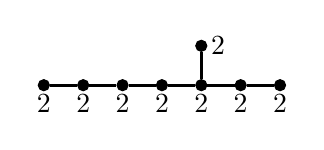
\begin{tikzpicture}
			\tikzset{dynode/.style={circle, draw, fill=black,
						minimum size=4pt, inner sep=0pt}}
			\tikzset{dyline/.style={line width=1pt}}
			\tikzset{dydash/.style={line width=1pt, dashed}}

			\begin{scope}[yshift=-10em, xshift=0]
				\node[dynode] (a1) at (0,0) {};
				\node[dynode] (a2) at (0.5,0) {};
				\node[dynode] (a3) at (1,0) {};
				\node[dynode] (a4) at (1.5,0) {};
				\node[dynode] (a5) at (2,0) {};
				\node[dynode] (a6) at (2.5,0) {};
				\node[dynode] (a7) at (3,0) {};
				\node[dynode] (a8) at (2,0.5) {};

				\draw[dyline] (a1) -- (a2) -- (a3) -- (a4) -- (a5) -- (a6) -- (a7);
				\draw[dyline] (a5) -- (a8);

				\node[below] () at (a1) {$2$};
				\node[below] () at (a2) {$2$};
				\node[below] () at (a3) {$2$};
				\node[below] () at (a4) {$2$};
				\node[below] () at (a5) {$2$};
				\node[below] () at (a6) {$2$};
				\node[below] () at (a7) {$2$};
				\node[right] () at (a8) {$2$};
			\end{scope}
		\end{tikzpicture}
		\quad\implies\quad
		\begin{pmatrix}
			2 & 1 &   &   &   &   &   &   \\
			1 & 2 & 1 &   &   &   &   &   \\
			  & 1 & 2 & 1 &   &   &   &   \\
			  &   & 1 & 2 & 1 &   &   &   \\
			  &   &   & 1 & 2 & 1 & 0 & 1 \\
			  &   &   &   & 1 & 2 & 1 & 0 \\
			  &   &   &   & 0 & 1 & 2 & 0 \\
			  &   &   &   & 1 & 0 & 0 & 2 \\
		\end{pmatrix}
	\]
	where each vertex of the tree is weighed by $2$.
\end{proposition}

It's interesting to note that if $Q$ is a matrix associated to a tree $T$, then $P(Q)$ has a $1$-skeleton homotopy equivalent to $T$. This connection between the $1$-skeleton and plumbing along a tree or graph was first noticed by Hirzebruch. It makes sense then why we'd care about matrices arising from trees instead of from general graphs which may contain cycles -- cycles break the simple-connectedness of the constructed manifold and are thereby much more complicated to work with.

% \begin{figure}[ht]\label{fig:negative-definite-trees}
% 	\centering
% 	\begin{tikzpicture}
% 		\tikzset{dynode/.style={circle, draw, fill=black,
% 					minimum size=4pt, inner sep=0pt}}
% 		\tikzset{dyline/.style={line width=1pt}}
% 		\tikzset{dydash/.style={line width=1pt, dashed}}
%
% 		\begin{scope}[yshift=0, xshift=22em]
% 			\node[dynode] (a1) at (0,0) {};
% 			\node[dynode] (a2) at (0.5,0) {};
% 			\node[dynode] (a3) at (1,0) {};
% 			\node[dynode] (a4) at (1.5,0) {};
% 			\node[dynode] (a5) at (2,0) {};
% 			\node[dynode] (a6) at (2.5,0) {};
% 			\node[dynode] (a7) at (3,0) {};
% 			\node[dynode] (a8) at (2,0.5) {};
%
% 			\draw[dyline] (a1) -- (a2) -- (a3) -- (a4) -- (a5) -- (a6) -- (a7);
% 			\draw[dyline] (a5) -- (a8);
%
% 			\node[] (l) at (1.75,-0.5) {$\E_8$};
% 		\end{scope}
%
% 		\begin{scope}[yshift=0, xshift=10em]
% 			\node[dynode] (a1) at (0,0) {};
% 			\node[dynode] (a2) at (0.5,0) {};
% 			\node[dynode] (a3) at (1,0) {};
% 			\node[dynode] (a4) at (1.5,0) {};
% 			\node[dynode] (a5) at (2,0) {};
% 			\node[dynode] (a6) at (2.5,0) {};
% 			\node[dynode] (a8) at (1.5,0.5) {};
%
% 			\draw[dyline] (a1) -- (a2) -- (a3) -- (a4) -- (a5) -- (a6);
% 			\draw[dyline] (a4) -- (a8);
%
% 			\node[] (l) at (1.5,-0.5) {$\E_7$};
% 		\end{scope}
%
% 		\begin{scope}[yshift=0, xshift=0]
% 			\node[dynode] (a1) at (0,0) {};
% 			\node[dynode] (a2) at (0.5,0) {};
% 			\node[dynode] (a3) at (1,0) {};
% 			\node[dynode] (a4) at (1.5,0) {};
% 			\node[dynode] (a5) at (2,0) {};
% 			\node[dynode] (a8) at (1,0.5) {};
%
% 			\draw[dyline] (a1) -- (a2) -- (a3) -- (a4) -- (a5);
% 			\draw[dyline] (a3) -- (a8);
%
% 			\node[] (l) at (1,-0.5) {$\E_6$};
% 		\end{scope}
%
% 		\begin{scope}[yshift=5em, xshift=3em]
% 			\node[dynode] (a1) at (0,0) {};
% 			\node[dynode] (a3) at (0.5,0) {};
% 			\node[dynode] (a4) at (1,0) {};
% 			\node[dynode] (a5) at (2.5,0) {};
% 			\node[dynode] (a6) at (3.0,0) {};
%
% 			\draw[dyline] (a1) -- (a3) -- (a4);
% 			\draw[dydash] (a4) -- (a5);
% 			\draw[dyline] (a5) -- (a6);
%
% 			\node[] (l) at (1.75,-0.5) {$\op{A}_n$};
% 		\end{scope}
%
% 		\begin{scope}[yshift=5em, xshift=17em]
% 			\node[dynode] (a1) at (0,0.4) {};
% 			\node[dynode] (a2) at (0,-0.4) {};
% 			\node[dynode] (a3) at (0.5,0) {};
% 			\node[dynode] (a4) at (1,0) {};
% 			\node[dynode] (a5) at (2.5,0) {};
% 			\node[dynode] (a6) at (3.0,0) {};
%
% 			\draw[dyline] (a1) -- (a3);
% 			\draw[dyline] (a2) -- (a3);
% 			\draw[dyline] (a3) -- (a4);
% 			\draw[dydash] (a4) -- (a5);
% 			\draw[dyline] (a5) -- (a6);
%
% 			\node[] (l) at (1.75,-0.5) {$\op{D}_n$};
% 		\end{scope}
% 	\end{tikzpicture}
% 	\vspace{1em}
% 	\caption{\todo{describe}}
% \end{figure}

\subsection{The Topology of Plumbed Manifolds}\label{sec:homotopy-type-plumbed}

In this section, we'll

\begin{proposition}
	If $\partial P^{2m}(Q)$ is a homotopy sphere then $Q$ is unimodular.
\end{proposition}

\begin{theorem}
	When $k>1$, $\partial P^{4k}(Q)$ is a homotopy sphere if and only if $Q$ is unimodular.
\end{theorem}


\begin{definition}
	The for $k>1$, the \defn{Milnor sphere} is the homotopy sphere $\partial P^{4k-1}(E_8)$.
\end{definition}

\subsection{Plumbing Constructions of 3-Manifolds}

Many of the results about the homotopy theory of plumbed manifolds in \cref{sec:homotopy-type-plumbed} only apply in dimensions $>4$. We can however still do the plumbing construction in $4$ dimensions, and it would be interesting to see what we get. In particular 

\todo{this section should be rewritten}

This $3$-manifold is known as (Poincar\'e) \defn{dodecahedral space} and has a beautiful geometric construction. We'll denote this space by $\mathscr{D}$. Aside from being a wonderful example of a non-Euclidean geometry, this space also was the first counter-example to an incorrect earlier form of the Poincar\'e hypothesised which stated that every homology $3$-sphere was also homeomorphic to the $3$-sphere. Much like exotic spheres are counter-examples to the smooth Poincar\'e hypothesis, in a similar vein the dodecahedral space can be thought of as a sort of ``proto exotic sphere'' serving as a counter-example to the ``proto Poincar\'e hypothesis''.

The classic construction of dodecahedral space $\mathscr{D}$ is due to Poincar\'e \todo{cite}. We begin by letting $\mathcal{D}\subset \R^3$ be a solid dodecahedron in three dimensional Euclidean space. The dodecahedron has 6 pairs of opposite pentagonal faces. Picking a clockwise spherical orientation on $\mathcal{D}$, we can glue together opposing faces with a minimal clockwise twist to line them up (see \cref{fig:dodecahedral_space_construction}). The resulting quotient space is a closed $3$-manifold, and this manifold is dodecahedral space $\mathscr{D}$.

\begin{figure}[ht]
	\centering
	\includegraphics[width=2in]{graphics/temp-diagrams/dodecahedral-space-geometric-construction.png}
	\caption{Construction of Dodecahedral Space}\label{fig:dodecahedral_space_construction}
\end{figure}

Given this geometric construction, it should be fairly straightforward -- albeit tedious -- to compute the homology of dodecahedral space by means of a cellular decomposition. After such a computation, we would find that:
\begin{proposition}
	Dodecahedral space is a homology $3$-sphere.
\end{proposition}

While the first homology of dodecahedral space is trivial and incapable of differentiating dodecahedral space from a 3-sphere, the fundamental group reveals a much richer geometric structure. If we let $\SO_3$ act on $\R^3$ in the usual way, we can form the symmetry group $\Sym(\mathcal{D})\subset \SO_3$ of orientation preserving orthogonal transformations which leave the dodecahedron $\mathcal{D}$ unchanged. This is known as the \defn{icosahedral group}\footnote{The icosahedron and dodecahedron are dual, so the choice of icosahedral in the name is purely a historical convention.} $\mathrm{I}\subset \SO_3$, a group containing $60$ elements and isomorphic to the alternating group $A_5$. There is a double cover of $\SO_3$ by the $\Spin_3$ Lie group:
\[
	\SU_2\cong \Spin_3\lkxto[2:1] \SO_3
\]
The \defn{binary icosahedral group}, denoted $2\mathrm{I}$, is the preimage of $\mathrm{I}$ under this double cover and hence contains $120$ elements. Since there is an exceptional isomorphism $\SU_2\cong \Spin_3$, the binary icosahedral group admits a representation by unitary complex $2\times 2$ matrices.
We then have:
\begin{proposition}
	The fundamental group of dodecahedral space is the binary icosahedral group.
\end{proposition}
This hints at another interesting fact about the binary icosahedral group -- it is a \defn{perfect group}, which means that it's commutator subgroup is the entire group. By the Hurewicz isomorphism, it would follow that
\[
	\H_1(\mathscr{D}) \cong \Ab\left[ \pi_1(\mathscr{D})\right] \cong 2\mathrm{I}/[2\mathrm{I}, 2\mathrm{I}] = 0
\]
where $\Ab$ denotes the abelianization. This perfectness of the fundamental group thus ``hides'' the non-trivial topology of $\mathscr{D}$ from being detectable by homology. It's interesting to note that dodecahedral space and $S^3$ are the only homology $3$-spheres up to homeomorphism with finite fundamental groups.

There is also a useful construction of dodecahedral space which will later appear in our later study of Brieskorn manifolds in \todo{cite}. If we identify $\SU_2$ with the $3$-sphere of unit quaternions, we obtain the construction:

\begin{proposition}
	There is a diffeomorphism $\mathscr{D} \cong S^3 / 2\mathrm{I}$ expressing dodecahedral space as the quotient of the $3$-sphere under a proper group action by $2\mathrm{I}$.
\end{proposition}

Finally, let's see how the dodecahedral space and binary icosahedral group arises out of the plumbing construction we've worked with thus far.

\todo{write this section}

\begin{proposition}
	There is a diffeomorphism $\mathscr{D}\cong \partial P^4(\E_8)$.
\end{proposition}

\todo{citations}

\begin{remark}
	In the early 2000's, the Wilkinson Microwave Anisotropy Probe (WMAP) was launched to accurately map out the cosmic microwave background, i.e. leftover heat from the Big Bang. The observed lack of temperature correlations above 60$^\circ$ led astrophysicist Jean-Paul Luminet to propose a cosmological model \cite{luminet2003dodecahedral} where the shape of the universe is a dodecahedral space, explaining the lack of large scale correlations by means of the compact topology of space. In such a finite universe, larger temperature correlations simply wouldn't have enough room to form.
	While this model made some predictions aligning with observed cosmological data
	\cite{roukema2008dodecahedral}, higher resolution data by the later Planck spacecraft later seemed to suggest that the observable large scale topology is trivial, leading to the modern prevalence of the $\Lambda$CDM model as a standard model for cosmology.
\end{remark}

\section{Surgery Theory}

Now that we have the basic constructions out of the way, let's \todo{introduce}

\subsection{Groups of Homotopy Spheres}

\begin{definition}
	\todo{groups of homotopy spheres}
\end{definition}

\subsection{Fundamental Theorems of Surgery}

\begin{definition}
	\todo{surgical invariant $\sigma$}
\end{definition}

\begin{theorem}[Plumbing Theorem]\label{thm:plumbing-theorem}
	When $m>2$, there is a normal map \[(g,c) : (W,\partial W) \to (D^{2m}, S^{2m-1})\] which restricts to a homotopy equivalence $g|_{\partial W} : \partial W \to  S^{2m-1}$ with the invariant $\sigma(g,c)$ taking on any integer value.
\end{theorem}

% \section{Complex Singularities}
%
% Let $F\in \C[z_0,z_1\ldots, z_n]$ be a non-constant polynomial in $(n+1)$-complex variables.
% \begin{definition}
% 	The \defn{variety} of $F$ is the complex hypersurface given by the zero locus
% 	\[
% 		\V(F) = F^{-1}(0)=\left\{ z \in \C^{n+1}  F(z)=0\right\} \subset \C^{n+1}.
% 	\]
% \end{definition}
%
% \todo{cauchy riemann equations}
%
% \begin{definition}
% 	The \defn{gradient} of a complex analytic function $F : \C^{n+1} \to \C$ is the $(n+1)$-tuple
% 	\[
% 		\nabla_F = \left(\frac{\partial F}{\partial z_0}, \frac{\partial F}{\partial z_1},\ldots, \frac{\partial F}{\partial z_n}\right).
% 	\]
% 	\todo{better definition}
% \end{definition}
%
% \begin{definition}
% 	A point $w\in \V(F)$ is a (complex) \defn{singularity}[complex singularity] if $\nabla_F(w)$ vanishes. A singularity is \defn{isolated}[isolated singularity] if there is a neighborhood surrounding $w$ which contains no other singularities.
% \end{definition}
%
% \begin{theorem}
% 	For small $\varepsilon>0$ the intersection of $\V(F)$ with $D_\varepsilon(w)$
% \end{theorem}
%
% \begin{proposition}
% 	Every sufficiently small sphere around an isolated singularity of $F$ intersects $\V(F)$ transversally in a smooth manifold.
% \end{proposition}
%
% \begin{definition}
% 	Let $w\in \V(F)$ be an isolated singularity. The \defn{link} of $F$ at $w$ is the intersection
% 	\[
% 		\L(F, w) = \V(F) \cap S^{2n+1}_\varepsilon(w) = \left\{ z\in \C^{n+1}  F(z)=0\textrm{ and } |z-w|<\varepsilon\right\}
% 	\]
% 	where $\varepsilon > 0$ is some sufficiently small real number so that $\L(F,w)$ is a smooth manifold intersecting the sphere $S^{2n+1}_\varepsilon(w)$ transversally.
% \end{definition}
%
% When the isolated singularity is clear, we write $\L(F)$.
%
% \subsection{Brieskorn Manifolds}
% The simplest examples of complex polynomials with isolated singularities are \todo{this}
%
% \begin{definition}
% 	Let $(a_0,a_1,\ldots, a_n)$ be an $(n+1)$-tuple of integers greater than or equal to $2$. The \defn{Brieskorn polynomial} of the tuple $(a_0,a_1,\ldots, a_n)$ is given by
% 	\[
% 		F(z_0,z_1,\ldots, z_n) = z_0^{a_0} + z_1^{a_1} +\cdots + z_n^{a_n}.
% 	\]
% 	Correspondingly, we refer to $\V(F)$ as the \defn{Brieskorn variety} of the tuple and to the link at the origin $\L(F,0)$ origin as the \defn{Brieskorn manifold}. We'll use the notation
% 	\[
% 		\Sigma(a_0,a_1,\ldots, a_n) =\L(z_0^{a_0}+z_1^{a_1}+\cdots+z_n^{a_n}, 0)
% 	\]
% 	to refer to these Brieskorn manifolds.
% \end{definition}
%
%
% \begin{proposition}
% 	If $p,q\geq 2$, then $\Sigma(p,q)\subset S^3$ is the torus link of type $(p,q)$.
% \end{proposition}
%
% \begin{proposition}
% 	There is a homeomorphism $\Sigma(2,2,2)\cong \RP^3$.
% \end{proposition}
%
% \begin{proposition}
% 	There is a homeomorphism $\Sigma(2,3,5)\cong \mathscr{D}$.
% \end{proposition}
%
% \subsection{The Fibration Theorem}
%
% \begin{theorem}\label{thm:fibration}
% 	If $F$ is a complex polynomial in $(n+1)$-variables with an isolated singularity at the origin, then there is a smooth fiber bundle map
% 	\[
% 		\lkxfunc{\phi}{S^{2n+1}_\varepsilon - \L(F)}{S^1}{z}{\arg F(z).}
% 	\]
% \end{theorem}
%
% For a given angle $e^{i\theta}\in S^1$, we'll denote the fiber of the bundle $\phi$ as $F_\theta = \phi^{-1}(e^{i\theta})$.
%
% \begin{proposition}
% 	Each fiber $F_\theta$ is a smooth parallelizable $2n$-manifold.
% \end{proposition}
%
% \subsection{When is the link a topological sphere?}
%
% Let's fix a polynomial $F$ in $(n+1)$ complex variables
%
% \begin{proposition}
% 	If $n\neq 2$, then $\L$ is homeomorphic to the sphere $S^{2n-1}$ if and only if $\L$ has the homology of a sphere. In fact, $\L$ is a topological sphere if and only if the reduced homology $\widetilde{H}_{n-1}(\L)$ is trivial.
% \end{proposition}
%
% Let's now choose an orientation for $F_\theta$.
%
% \begin{proposition}
% 	The manifold $\L$ is a homology sphere if and only if the intersection form
% 	\[
% 		\lkxfunc{Q_{F_\theta}}{\H_n(F_\theta)\times \H_n(F_\theta)}{\Z}
% 	\]
% 	has determinant $\pm 1$ -- in other words if $Q_{F_\theta}$ is unimodular.
% \end{proposition}
%
% \section{Kervaire Invariant}
%
% \begin{theorem}[Brieskorn-Pham]
% \end{theorem}
%
% \begin{theorem}[Levine]
% 	If $n$ is odd, the Kervaire invariant is given by
% 	\[
% 		c(F_0) = \begin{cases}
% 			0 & \textrm{if }\Delta(-1)\equiv \pm 1\mod 8 \\
% 			1 & \textrm{if }\Delta(-1)\equiv \pm 3\mod 8
% 		\end{cases}
% 	\]
% \end{theorem}
%
% \begin{theorem}[Hirzebruch-Mayer] Smooth Brieskorn varieties are parallelizable.
% \end{theorem}


\chapter{Classification of Homotopy Spheres}\label{chap:classification}
\chapter{Classification}\label{chap:classification}

\section{Surgery Theory}

\section{Kervaire-Milnor Theorem}

\section{Kervaire Invariant}

\section{Very Exotic Spheres}


\begin{appendices}
\chapter{Differential Geometry}\label{chap:differential_geometry}
\begin{flushleft}
	\textsl{I admire the elegance of your method of computation;}\\
	\textsl{it must be nice to ride through these fields upon the}\\
  \textsl{horse of true mathematics while the like of us have to}\\
  \textsl{make our way laboriously on foot.}\\
	\rule[0pt]{24em}{0.5pt}\\
	-- \textsc{Albert Einstein} to \textsc{Tullio Levi-Civita}\\
	\vspace{2em}
\end{flushleft}

\begin{definition}\label{defn:manifold_structure}
  Let $(G,\rho)$ be an $n$-dimensional symmetry type and suppose $X$ is an $n$-dimensional manifold with frame bundle $\varpi : \B X \to X$. A \defn{$(G,\rho)$-structure} on $X$ is a reduction of $\varpi$ along the representation $\rho : G \to \GL_n$.
\end{definition}

\section{Lie Groups and Lie Algebras}

\section{Connections on Principal Bundles}


\chapter{Characteristic Classes}\label{chap:characteristic_classes}
% \section{The Chern-Weil Homomorphism}

\section{Chern and Pontryagin Classes}

\begin{proposition}\label{prop:pontryagin_classes_of_CPn}
  The Pontryagin classes of complex projective space $\CP^n$ are
  \[
    p_k(\CP^n) = \binom{n+1}{k}\quad\textrm{for}\quad 1\leq k \leq n/2.
  \]
\end{proposition}

\section{Stiefel-Whitney Classes}\label{sec:stiefel-whitney_classes}

\section{Universal Bundles}\label{sec:universal_bundles}

\todo{"the most twisted bundle" from Bott and Tu}
\cite{milnorstasheff1974characteristic}
\cite{botttu1982differential}

\begin{theorem}\label{thm:cohomology_of_BO}
  There is a ring isomorphism
  \[
    \H^\bullet(\BO_n; \Z/2) \cong \Z/2[w_1,\ldots, w_n]
  \]
  where $w_i$ are Stiefel-Whitney classes of the universal bundle over $\BO_n$. In other words, any characteristic class for unoriented real bundles with $\Z/2$-coefficients can be expressed in terms of the Stiefel-Whitney classes.
\end{theorem}

\begin{theorem}\label{thm:cohomology_of_BSO}
  Let $\Lambda$ be an integral domain containing $1/2$. There are ring isomorphisms
  \[
      \H^\bullet(\BSO_{2m+1}; \Lambda) \cong \Lambda[p_1, \ldots, p_m]
      \quad\textrm{and}\quad
      \H^\bullet(\BSO_{2m}; \Lambda) \cong \Lambda[p_1, \ldots, p_m, e]/(e^2-p_m)
  \]
  where $p_i$ and $e$ are Pontryagin and Euler classes of the universal bundle over $\BSO_n$.
  In other words, ignoring $2$-torsion, any characterstic class for oriented real bundles can be expressed in terms of Pontryagin and Euler classes.
\end{theorem}


\chapter{Cobordism}\label{chap:cobordism}
\section{Thom-Pontryagin Construction}\label{sec:thom-pontryagin_construction}

\section{The Rational Oriented Cobordism Ring}

\begin{theorem}[Thom-Pontryagin]\label{thm:thom-pontryagin_oriented_cobordism}
  The following holds:
  \begin{enumerate}
    \item There is a ring isomorphism $\Omega^\SO_\bullet \cong \pi_\bullet \MSO$.
    \item There is a ring isomorphism $\pi_\bullet\MSO \otimes \Q \cong \H_\bullet(\BSO; \Q)$.
    \item We have $\H_\bullet(\BSO; \Q) \cong \Q[p_1, p_2,\ldots]$ where $|p_i|=4i$.
  \end{enumerate}
  Putting this all together, there is a ring isomorphism
  \[
    \Omega^\SO_\bullet\otimes \Q \lkxto[\cong] \Q[[\CP^2], [\CP^4],\ldots]
  \]
  where $[\CP^{2n}]$ are oriented cobordism classes of complex projective planes.
\end{theorem}
\begin{proof}
\end{proof}


\chapter{Index Theory}\label{chap:index_theory}

\section{The Hirzebruch Signature Theorem}

\begin{theorem}[Hirzebruch Signature Theorem]\label{thm:hirzebruch_signature}
  \todo{todo}
\end{theorem}

\begin{proof}
\end{proof}

\subsection*{Harmonic Forms}

Given a function $\psi : U \to \R$ on an open region of $\R^n$, the Laplace equation\index{Laplace equation} is the second-order partial differential equation
\begin{equation}\label{eq:laplace}
    \Delta \psi = 0
    \quad\implies\quad
    \frac{\partial^2 \psi}{\partial x_1^2}+\cdots+\frac{\partial^2 \psi}{\partial x_n^2}=0.
\end{equation}
Functions satisfying this equation are known as \defn{harmonic functions}[harmonic function] and are ubiquitous across mathematics and physics. The Laplacian operator $\Delta$

\section{The Atiyah-Singer Index Theorem}

\begin{theorem}[Atiyah-Singer Index Theorem]\label{thm:atiyah-singer_index}
  Let $X$ be a closed oriented $n$-manifold and let $(E,D)$ be an elliptic complex on $X$. Then we have
  \[
    \ind(E, D) = (-1)^{n(n+1)/2}\int_X \mathrm{ch}(E,D)\smile \Td(\T X_\C).
  \]
\end{theorem}


\chapter{Homotopy Groups of Spheres}\label{chap:homotopy_groups_of_spheres}
\input{chapters/homotopy_groups_spheres}
\end{appendices}

\lkxrefs
\lkxindex

\end{document}
